    \chapter{Introduction to Differential Equations}
    
        Roughly stated, differential equations is the study of a system that undergoes change.  This change can depend on time, space, or both.  The history of differential equations begins with Newton's study of classical mechanics.  Newton was investigating the motion of objects in space and derived the first examples of differential equations.  The field quickly grew with the once other scientists noticed the wide scope of applicability of differential equations.  
        
        In the time of Newton's classical mechanics, we saw the advent of celestial, fluid, and continuum mechanics. Examples include the diffusion, advection, and wave equations.  Other fields of science began to use these ideas from physics to model population dynamics and chemical reaction.  As time moved forward, more complicated physical interactions brought even more uses of differential equations to the forefront.  These were the dyanamical theories of electromagnetism and thermodynamics.  All of this happened before the turn of the 20$^\textrm{th}$ century.
        
        As we moved into the 1900s, there was the boom of modern physics with work from Einstein and many other scientists.  Einstein described the motion of atoms in a probabalistic manner that was also deeply related to differential equations of classical mechanics.  Soon after, he then  considered how spacetime itself behaves as a coupled dyanamical continuum, much like the head of a drum that vibrates.  It was shortly after this discovery that Sch\"odinger and Heisenberg independently developed the theories of quantum mechanics.  Both stated the problem in different (but equivalent) ways.  This study brought together the notion of motion of particles with that of waves.
        
        Time passed, and in the mid 1900s computers were developed.  This forever changed the study of differential equations.  The problem was, we were finding that (other than very specific nice examples) most differential equations were extremely hard to solve.  In fact, many are so wild that the dynamics we see is volatile to the point of the so called ``butterfly effect."  These volatile systems are known as chaotic and are abundant in nature.  Weather, population, and chemical reaction are all areas where chaos can show up.  However, the ability to approximate solutions with computers allows us to make reasonable predictions and essentially solve problems that were previously deemed impossible.
        
        The goal for us is not to learn to solve many differential equations with a handbook of techniques.  These techniques can be readily found online and are very formulaic.  If you do them once, you can do them again.  Instead, our goal is to understand what differential equations model and what they say about systems.  Of course, we will explicitly solve some and see a few techniques, but that is not the emphasis.  If one pursues mathematical modelling, one will almost surely be working with computers to solve problems rather than by hand. It is with this mentality that we carry on to uncovering this structure of differential equations.
        
        \section{Ordinary Differential Equations}
        
        The first stop on the study of differential equations are the Ordinary Differential Equations (ODE).  ODE are equations that involve a single variable $t$ that we usually think of as time, a function $f(t)$, and derivatives of the function $f'(t)$, $f''(t)$, $f'''(t)$, up to $n$ derivatives $f^{(n)}(t)$.  We will not worry ourselves with the higher order equations yet, as we will find they break down into lower order equations.
        
        Unlike previous problems where we solve for a variable, or compute derivatives, we wish to find a function that satisfies the differential equation.  So, our aim is to find $f(t)$ given our understanding of how $f$ changes over time.
        
        \begin{ex}{First Order ODE}{first_order}
        Suppose we are asked to find a function $f(t)$ that satisfies the following relationship (ODE):
        \[
        f'(t) = g(t,f(t)).
        \]
        This is an example of the most general \emph{first order} ODE. 
        \begin{itemize}
            \item Written in english, this equation says, ``what function $f(t)$ has a derivative that is equal to a function of $t$ and $f(t)$?"
            \item Though confusing at first, this ends up becoming very natural.
        \end{itemize}
        \end{ex}
        
        \begin{df}{Order of an ODE}{order}
        The \textbf{order} of an ODE is the highest derivative that appears in the ODE.
        \end{df}
        
        \begin{ex}{Exponential Growth and Decay}{exp_growth_decay}
        As opposed to a very general set up, let us consider the following problem statement.
        
        \emph{The concentration of Plutonium in a vessel is measured over time.  It's found that the rate of change of this concentration is proportional to the current concentration.  What ODE models this situation?}
        
        The answer to the above question is
        \[
        f'(t)=kf(t).
        \]
        \begin{itemize}
            \item We let $f(t)$ represent the concentration of Plutonium at time $t$.
            \item The rate of change of $f$, $f'(t)$, is related to the current concentration $f$ by a proportion $k$.
        \end{itemize}
        \end{ex}
        
        \begin{ex}{Mechanical Law in $3D$}{mechanical_law}
        Newton's study of the motion of bodies brought him to say the following.
        
        \emph{The change in velocity of a body is proportional to the force applied divided by the inertial mass of the body.}
        
        The equation that models this is
        \[
        \mathbf{v}'(t)=\frac{1}{m} \mathbf{F}(t).
        \]
        \begin{itemize}
            \item The $\mathbf{v}$ represents the body's velocity at the time $t$ and thus $\mathbf{v}'$ is the change in velocity.
            \item The change in velocity should be equal to the applied force, $\mathbf{F}(t)$ but also dependent on the objects mass $m$.
            \item We could also describe this equation by noting the fact that $\mathbf{v}$ is the derivative of the position $\mathbf{x}$. This gives
            \[
            \mathbf{x}''(t)=\frac{1}{m}\mathbf{F}(t).
            \]
        \end{itemize}
        \end{ex}
        
        \begin{ex}{Harmonic Motion in $1D$}{harmonic_motion}
        There are many systems that are not first order.  For example, we might have the following.
        
        \emph{A spring has a rest length $L$. The force on a mass on a spring is proportional to the displacement from this rest length $L$ in the direction opposite the displacement. The force causes an acceleration proportional to the force applied dived by the inertial mass of the body.}
        
        The governing ODE is
        \[
        y''(t) = -\frac{k}{m}(y(t)-L).
        \]
        \end{ex}
        
        \section{Solutions to an ODE}
        
        What do we mean when we say that we want to ``solve an ODE?" This means we want to find a function whose derivatives satisfy our ODE.  Let us see a few examples.
        
        \begin{ex}{Exponential Growth and Decay Solution}{exp_growth_decay_solution}
        Previously, we were given the equation
        \[
        f'(t)=kf(t).
        \]
        I claim that 
        \[
        f(t)=Ae^{kt}
        \]
        is a solution to this ODE for any choice of $A$. 
        
        We take 
        \[
        f'(t)=\frac{d}{dt}(Ae^{kt})=Ake^{kt}=kf(t),
        \]
        so indeed $f(t)$ is a solution.
        \end{ex}
        
        \begin{ex}{Mechanical Law in $3D$ Solution}{mechanical_law_solution}
        Let us suppose that there is no force acting on the object.  We should all believe the object should move in a straight line.  With the condition of no force, the equation reads
        \[
        \mathbf{v}'(t)=\mathbf{0}.
        \]
        I claim that 
        \[
        \mathbf{v}(t)=\begin{bmatrix} c_1 \\ c_2 \\ c_3 \end{bmatrix}
        \]
        with $c_1, c_2$ and $c_3$ constants, is a solution to this equation. 
        
        So we take
        \[
        \mathbf{v}'(t)=\frac{d}{dt} \begin{bmatrix} c_1 \\ c_2 \\ c_3 \end{bmatrix} = \begin{bmatrix} 0 \\ 0 \\ 0 \end{bmatrix} = \mathbf{0}.
        \]
        Indeed, this is a solution.  The solution is that of a straight line in space.  We can see this more easily by noting we also have the ODE
        \[
        \mathbf{x}'(t) = \mathbf{v}(t).
        \]
        Again, I claim that
        \[
        \mathbf{x}(t) = \begin{bmatrix} c_1 t \\ c_2 t \\ c_3 t\end{bmatrix}
        \]
        is a solution that is a straight line in space.
        \end{ex}
        
        \begin{exercise}
        Verify that $\mathbf{x}(t)$ above is indeed a solution to 
        \[
        \mathbf{x}'(t)=\mathbf{v}(t).
        \]
        \end{exercise}
        
        \begin{ex}{Harmonic Motion in $1D$ Solution}{harmonic_motion_solution}
        We were given the following
        \[
        y''(t) = \frac{-k}{m} (y(t)-L).
        \]
        This equation, being second order, is immediately more difficult to solve.  What we can do, however, is make a change of variables to
        \[
        x(t)=y(t)-L
        \]
        and note that
        \[
        x''(t)=y''(t)
        \]
        but the ODE changes to
        \[
        x''(t)=\frac{k}{m}x(t).
        \]
        This is much easier to solve.  The idea of changing variables is extremely helpful.
        
        In these new variables, we can see the following figure.
        \begin{figure}[H]
            \centering
            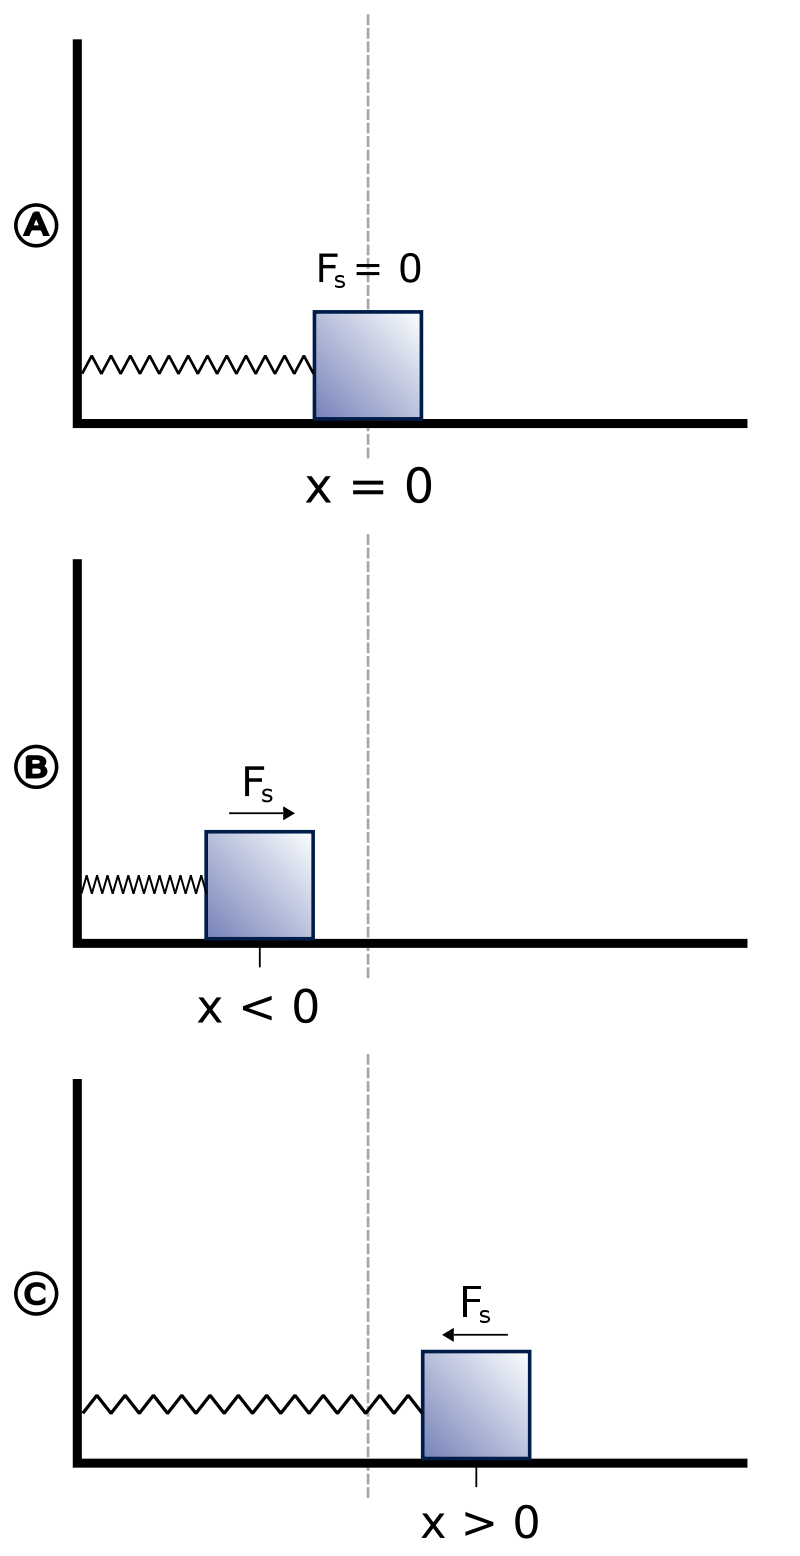
\includegraphics[width=.4\textwidth]{Figures/spring-mass.png}
            \caption{Spring-Mass system in the new variables. The dashed line represents the rest length $L$.}
            \label{fig:my_label}
        \end{figure}
        \end{ex}
        
        \begin{exercise}
        Show that
        \[
        y(t) = A\sin\left(\sqrt{\frac{k}{m}}t\right)+B\cos\left( \sqrt{\frac{k}{m}}t\right)
        \]
        solves the above differential equation.
        \end{exercise}
        
        \section{Separable ODE}
        The nicest possible ODE come from equations that are \emph{separable}.  What this means is that, for example, we have a first order equation like
        \[
        f'(t)=g(t)h(f(t)).
        \]
        Why is this nice? Well, in particular, it means that we can simply integrate this equation to solve it.  Many systems exhibit symmetry that allows for this type of separation, so this technique is crucial.
        
        In general, we have
        \[
        f'(t)=\frac{df}{dt}
        \]
        and we put
        \begin{align*}
            \frac{df}{dt}&=g(t)h(f(t))\\
            \iff \frac{1}{h(f(t))}df &= g(t)dt.
        \end{align*}
        With this, we can integrate both sides, then solve for $f$.  
        
        \begin{ex}{Separable ODE}{separable}
        Consider the following ODE
        \[
        f'(t)=\frac{t}{f(t)}. 
        \]
        Then we can put
        \begin{align*}
            \frac{df}{dt}&= \frac{t}{f}\\
            \iff fdf &= t dt.
        \end{align*}
        Then we can take the antiderivative of both sides and find
        \begin{align*}
            \int fdf &= \int t dt\\
            \iff \frac{1}{2}f^2 &= \frac{1}{2}t^2 + C\\
            \iff f(t)&=\sqrt{t^2+2C}.
        \end{align*}
        So now we can verify that this is in fact a solution to our ODE.  So we take
        \[
        f'(t) = \frac{d}{dt}\sqrt{t^2+2C}= \frac{t}{\sqrt{t^2+2C}} = \frac{t}{f(t)}.
        \]
        \end{ex}
        
        \begin{exercise}
        Solve the following ODE using separation
        \[
        f'(t)=t.
        \]
        Note that there will be an undetermined constant that we will learn how to handle next.
        \end{exercise}
        
        \section{Particular Solutions}
        In all previous examples, there were undetermined constants.  These constants appear since fundamentally an antiderivative is determined up to a constant.  Though not all ODE are solvable by direct integration, the constants are there due to this reason.
        
        How do we determine the constants?  It turns out we need a bit more information.  The extra information is also very intuitive and physical.  Take for example, a simplified version of the harmonic oscillator (spring-mass) system
        \[
        x''(t) = -x(t).
        \]
        Notice, we have just removed the constants.  This is always possible to do by picking the right way to measure the problem! Then I stated that the \emph{general solution} to this ODE is
        \[
        x(t)=A\sin(t) + B \cos (t).
        \]
        But, we don't know $A$ and $B$.  
        
        \begin{df}{General Solution}{gen_soln}
            A \textbf{general solution} to an $n$th order ODE is a solution with $n$  (call these values $c_1,c_2,\dots,c_n$) undetermined constants. A general solution is in fact a whole family of solutions. That is, there is a solution for each different value of the constants $c_1$, $c_2$, $\dots$, $c_n$.
        \end{df}
        
        If we think about the situation, we have just determined the general oscillatory behavior of the system, but not the any particular \emph{trajectory} of the system. What we need to know is where we pulled the mass to at the initial time $t=0$. That is, we need
        \[
        x(0)
        \]
        but we also need to know how fast it was moving at that point 
        \[
        x'(0).
        \]
        The analogy is as follows: If one is throwing a ball, one needs to know where it is released $\mathbf{x}(0)$, and the velocity at which it is released at $\mathbf{x}(0)$ in order to know where the ball will land.
        \begin{figure}[H]
            \centering
            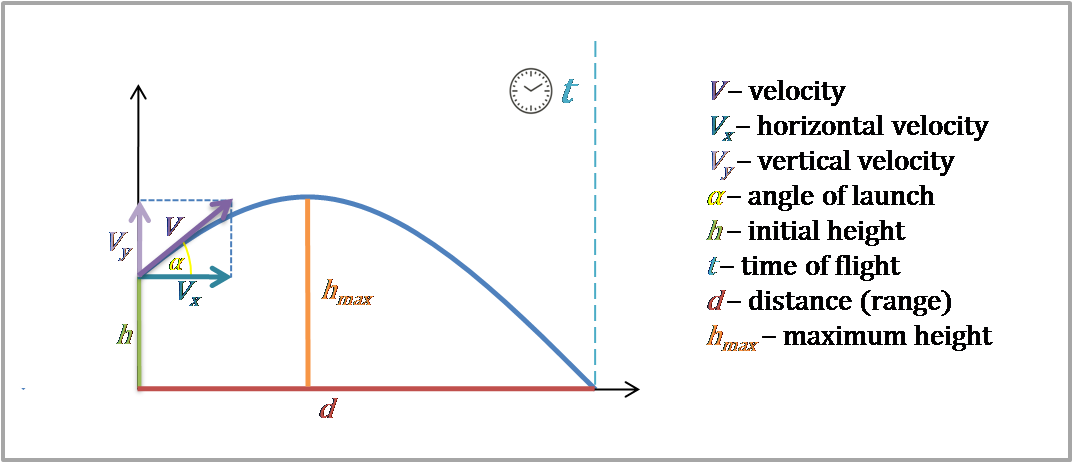
\includegraphics[width=.7\textwidth]{Figures/projectile-motion.png}
            \caption{Throwing a ball as an example of needing initial data.}
            \label{fig:my_label}
        \end{figure}
        We call these values $x(0)$ and $x'(0)$ the \emph{initial data}. 
        
        \begin{df}{Initial Data}{df: initial_data}
            The \textbf{initial data} to an $n$th order ODE are the specific values for
            \[
            x(0),~ x'(0),\dots,~ x^{(n-1)}(0),
            \]
            where $x^{(k)}$ represents the $k$th derivative of $x(t)$.
        \end{df}
        
        \begin{df}{Particular Solution}{particular_solution}
            A \textbf{particular solution} is one member of the family of general solutions.  That is, a solution where the constants $c_1,~c_2,\dots,~c_n$ are all uniquely determined.
        \end{df}
        
        \begin{prop}{Initial Data and Particular Solutions}{initial_data_part_solns}
        In order to find a particular solution to an $n$th order ODE, one needs to know the initial values of the function, its derivative, its second derivative, and all derivatives up to the $(n-1)th$ derivative
        \[
        x(0),~ x'(0),\dots,~ x^{(n-1)}(0).
        \]
        \end{prop}
        
        
        
        \begin{ex}{Particular Solution to Harmonic Oscillator}{part_soln_harm_osc}
        Consider 
        \[
        x''(t)=-x(t)
        \]
        with initial data
        \[
        x(0)=1, ~ x'(0)=0.
        \]
        This has the general solution
        \[
        x(t)=A \sin(t) + B \cos (t).
        \]
        We can find the particular solution by
        noting we have
        \[
        x(0)=A\sin(0)+B\cos(0)=1
        \]
        from our initial data.  Specifically, this gives us that
        \[
        B=1.
        \]
        Then note we also have
        \[
        x'(0)=A\cos (0) - \sin (0)=0
        \]
        which gives us that
        \[
        A=0.
        \]
        So our particular solution is
        \[
        x(t)=\cos (t).
        \]
        \end{ex}
        
        \subsubsection{Determinism}
        The reason why we study these differential systems is to make predictions and models.  Given that, our predictions must be sensible. This means if we are given a differential equation and initial data, there should only be one particular solution.  This is known as \textbf{determinism}.  
        
        Not all systems are deterministic.  But it turns out the non-deterministic systems are either problematic as models or just very hard to deal with.
        
        When solving an ODE, we call a particular solution a \textbf{trajectory}.
        
        
        \section{Projectile Motion}
        Above, we saw the example picture of projectile motion.  We have all thrown a ball, and we know what the motion looks like.  Let us derive exactly the equations of motion of a thrown ball and then a specific trajectory.
        
        \begin{ex}{Projectile Motion in 1D}{1d_proj_motion}
        Here we will start from a physical postulate, create a differential equation model, solve the model in general, then in particular, and lastly plug in exact values and units.
        
        \noindent \textbf{Problem Statement:} \emph{Near Earth, gravity is constantly forcing objects to accelerate downward at a constant rate $g=9.8m/s^2$. What is the trajectory of a ball with mass $5kg$ thrown straight upward from a height of $1m$ with initial velocity $10m/s$?}
        
        Since we only care about the ball moving straight up and down, we need only describe the height.  We let the height be given by $z(t)$ and acceleration is then the second derivative of height $z''(t)$.  We are told that the acceleration is downward at some constant rate, say $g$.  It turns out, the mass does not change this acceleration and we arrive at the equation
        \[
        z''(t)=-g
        \]
        where the minus sign tells us the object accelerates downward.
        
        It turns out this equation is separable, but requires a bit more care.  Note we have
        \[
        \frac{d^2z}{dt^2}=\frac{d}{dt}\frac{dz}{dt}=-g.
        \]
        The fundamental theorem of calculus says that we can take the antiderivative of this equation and get
        \[
        \frac{dz}{dt}=-g+C_1.
        \]
        Now we separate and integrate,
        \[
        \int dz = \int (-gt+C_1)dt
        \]
        and get
        \[
        z= -\frac{1}{2}gt^2+C_1t+C_2.
        \]
        So our general solution is
        \[
        z(t)=-\frac{1}{2}gt^2+C_1t+C_2.
        \]
        
        Then, say we are given initial data
        \[
        z(0)=z_0 \qquad z'(0)=z_1
        \]
        then using our general solution we have
        \[
        z(0)=-\frac{1}{2}g(0)^2+C_1(0)+C_2=z_0
        \]
        so 
        \[
        C_2=z_0.
        \]
        Then we can again use the general solution and get
        \[
        z'(0)=-g(0)+C_1 = z_1
        \]
        so
        \[
        C_1 = z_1.
        \]
        So our particular solution is then
        \[
        z(t) = -\frac{1}{2}gt^2 + z_1 t + z_0.
        \]
        
        Looking again at our problem statement, we are given that our initial height is
        \[
        z(0)=1m=z_0
        \]
        and the initial velocity is
        \[
        z'(0)=10m/s = z_1,
        \]
        So with our specific problem, the \textbf{trajectory} is
        \[
        z(t)=-\frac{1}{2}(9.8)t^2 + 10t+1.
        \]
        Here is the plot of this trajectory.
        \begin{figure}[H]
            \centering
            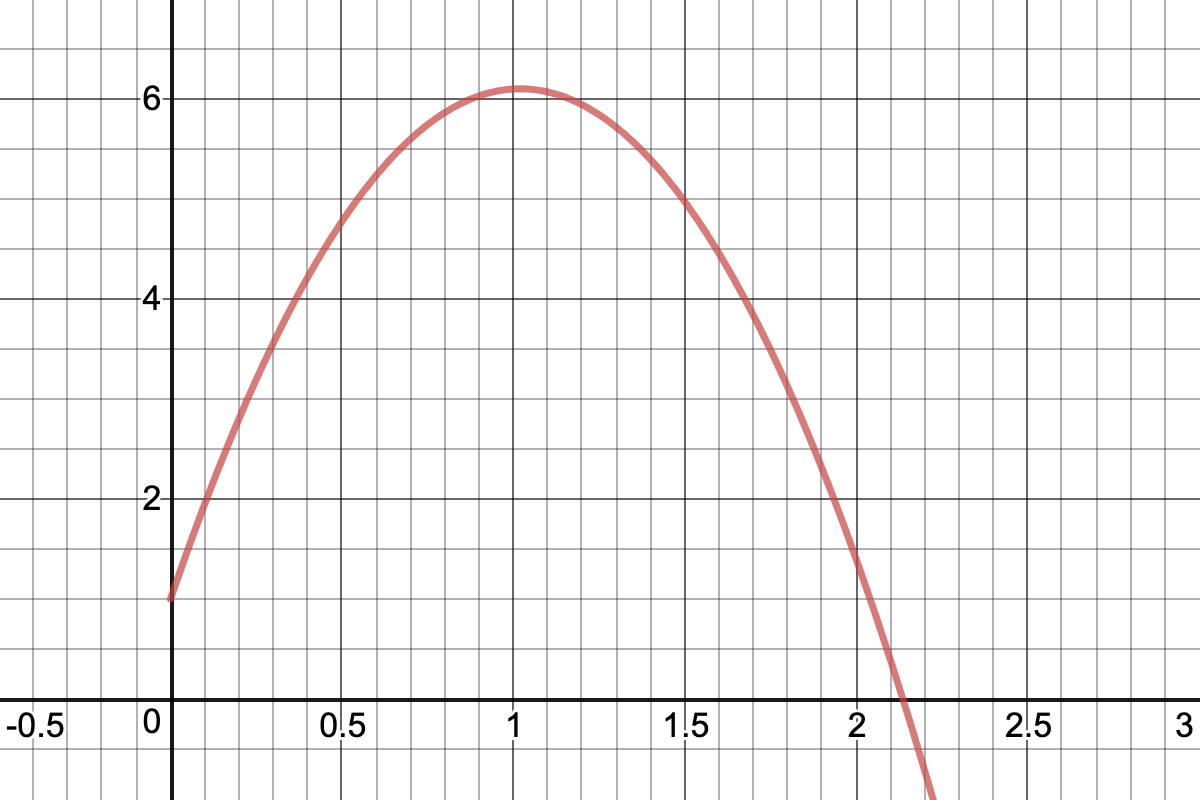
\includegraphics[width=.7\textwidth]{Figures/projectile_example.png}
            \caption{The trajectory of our example ball.}
            \label{fig:my_label}
        \end{figure}
        Notice that at some point this ball would go below the ground!  Our models aren't all knowing.  You would have to impose more information on the problem to say that the ball cannot go through $z=0$!  This goes to show that our models tend to only work over a short span in time. Even for a relatively simple problem like throwing a ball, we still have issues.
        \end{ex}
        
        \section{Exact Equations}
        
        To extend to a slightly larger class of equations, we consider one more type of first order equation.  These are the \emph{exact} equations.  These are differential equations that are much like the potential functions we saw in Part II.  We are given an equation
        \[
        P(x,t)dx + Q(x,t)dt = 0.
        \]
        Note that this is equivalent to a first order differential equation by rearranging
        \begin{align*}
            P(x,t)dx+Q(x,t)dt &= 0 \\
            \iff P(x,t)dx &= - Q(x,t)dt\\
            \iff \frac{dx}{dt} &= \frac{-Q(x,t)}{P(x,t)}\\
            \iff x' &= f(x,t).
        \end{align*}
        Exact equations make their appearance often in thermodynamics (with entropy, for example) but are in fact very far reaching.  One can understand complicated \emph{partial differential equations} by generalizing this concept.
        
        \begin{df}{Exact ODE}{exact}
        A first order equation 
        \[
        P(x,t)dx + Q(x,t)dt = 0
        \]
        is \textbf{exact} if there exists an $F(x,t)$ such that
        \[
        \frac{\partial F}{\partial x}= P(x,t) \quad \textrm{and} \quad \frac{\partial F}{\partial t}= Q(x,t).
        \]
        \end{df}
        
        \begin{prop}{An Equivalent Definition for Exactness}{exactness_equivalent}
        A first order equation
        \[
        P(x,t)dx + Q(x,t)dt = 0
        \]
        is exact if and only if
        \[
        \frac{\partial P}{\partial t}-\frac{\partial Q}{\partial x}=0.
        \]
        \end{prop}
                
        We can solve an exact equation in an analogous way to solving for a potential function.  Let us see where this comes from a bit.
        
        Let's say we have a function $F(x,t)$.  Then, the level curves of this function $F(x,t)=c$ can be thought of as trajectories!  
        
        \begin{ex}{Exact: Forward and Back}{exact_forward_back}
        \noindent \textbf{Forward:}
        Let's consider the function
        \[
        F(x,t) = x^2+t^2.
        \]
        Then a level curve is given by
        \[
        F(x,t)=x^2+t^2 = c
        \]
        which is a circle of radius $\sqrt{c}$.  Often times knowing this is the closed trajectory is enough.  For example, in the case for finding orbits of the planets.
        
        Then we can take what is called the \emph{differential} of both sides
        \begin{align*}
        dF(x,t)&=dc\\
        \implies \frac{\partial F}{\partial x}dx + \frac{\partial F}{\partial t}dt &= 0.
        \end{align*}
        Now, with our particular case we have
        \[
        2xdx+2tdt = 0.
        \]
        Is this equation exact? Yes, by definition, it is.  But we should verify with the proposition.  So we let
        \[
        P(x,t) = 2x \quad \textrm{and} \quad Q(x,t) = 2t
        \]
        and compute the partial derivatives
        \[
        \frac{\partial P}{\partial t} = 0 \quad \textrm{and} \quad \frac{\partial Q}{\partial x} = 0
        \]
        so indeed this proposition holds.
        
        \noindent \textbf{Back:} Say we were given
        \[
        2xdx+2tdt = 0, 
        \]
        how do we recover $F(x,t)$?  Can we recover it exactly?  Let's see.
        
        Here we can integrate the $dx$ term with respect to $x$ and determine a function up to an additional $f(t)$
        \[
        \int 2xdx = x^2 + f(t).
        \]
        Similarly, we can integrate the $dt$ term with respect to $t$ and find
        \[
        \int 2tdt = t^2 + g(x).
        \]
        Combining these two, we find that we have
        \[
        H(x,t) = x^2+t^2+c.
        \]
        However, we cared just about the level curves of this function so really, we recover
        \[
        x^2+t^2=c.
        \]
        \end{ex}
    
        \chapter{Systems of ODE}
        Though ODE consist of a single variable, it's possible that many ODE interact with each other and form a system.  Another case of interest would be finding trajectories as curves in higher dimensions (usually 2 or 3 for physical problems).  In this case we say that we have an \emph{system of ODE}.  
        
        For example, a system of three first order ODEs takes the form
        \begin{align*}
            x' &= f(x,y,z,t),\\
            y' &= g(x,y,z,t),\\
            z' &= h(x,y,z,t).
        \end{align*}
        
        \begin{df}{System of ODE}{system_of_ode}
            A \textbf{system of ODE} is a collection of differential equations of various order.  We call the system \textbf{coupled} if one of the differential equations is dependent on another.
        \end{df}
        
        \begin{ex}{SIR Model in Ecology}{sir_model}
        A biological example of a system of first order equations comes from modeling the spread of disease in a colony.  We let $S(t)$ denote the number of susceptible animals, $I(t)$ denote the number of infected animals, and $R(t)$ denote the animals resistant to the disease.  The model is a system of ODE of the form
        \begin{align*}
            S' &= -\frac{\beta IS}{N},\\
            I' &= \frac{\beta I S}{N} - \gamma I,\\
            R' &= \gamma I.
        \end{align*}
        We let $N=S(t)+I(t)+R(t)$ denote the constant population, and $\beta$ and $\gamma$ are other measured parameters.
        
        This is a coupled system since, for example, the equation $S'$ contains the function $I$.  We also see that the equation for $I'$ contains the function $S$.  Lastly, the equation for $R'$ contains the function $I$.  
        \end{ex}
        
 
        
        \section{Qualitative Analysis}
        The great part about a system of first order ODEs is that we can analyze them pictorially. 
        
        \begin{ex}{Zoo of First Order Linear Systems}{first_order_zoo}
        Let's consider the following systems.
        
        \begin{enumerate}[(I)]
            \item 
            \begin{align*}
                x' = x+y,\\
                y' = x+y.
            \end{align*}
            What we can do is put $x'$ and $y'$ into a vector 
            \[
            \mathbf{v}' = \begin{bmatrix} x' \\ y' \end{bmatrix}.
            \]
            This is actually a vector field $\mathbf{v}'(x,y)$!  We can plot this vector field and analyze from there.
            \begin{figure}[H]
                \centering
                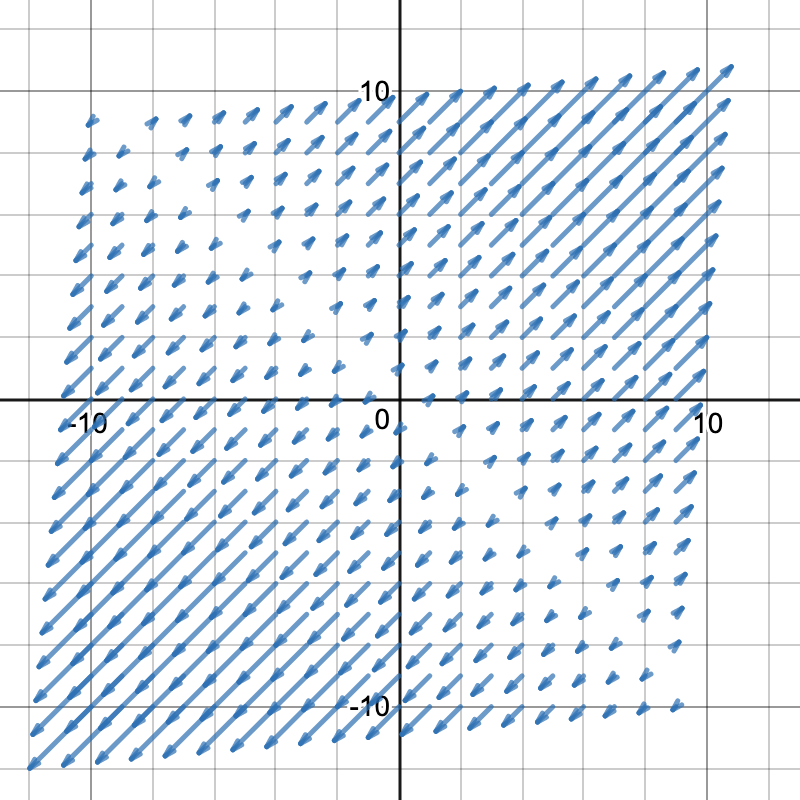
\includegraphics[width=.6\textwidth]{Figures/x+yx+y.png}
                \caption{A plot of the vector field $\mathbf{v}'(x,y)$.}
            \end{figure}
            Our goal is to then find a vector as a function of time given by
            \[
            \mathbf{v}(t) = \begin{bmatrix} x(t) \\ y(t) \end{bmatrix}
            \]
            as this will contain the solutions to our system of ODE.
            
            What we do next is pick an initial condition, $(x_0,y_0)$ and note that our vector field gives us the velocity vector $\mathbf{v}'(x_0,y_0)$ at that point. 
            
            The solution (curve/trajectory) to our system of ODE follows the vector field above since it describes the velocity of our curve at that point. We call this solution curve an \textbf{integral curve} as it is obtained (roughly) through integration of $\mathbf{v}'$.  However, you should know that it is not always possible to explicitly compute this integral.  We will learn techniques for solving certain systems, however.
            
            One should feel comfortable tracing an estimate for a solution curve for a given system as it gives a qualitative answer to the problem. In this case, if we pick a point along the line $y=-x$, the trajectory is stationary.  Otherwise, the solution follows a curve that is parallel to the $y=x$ line and the direction depends on which location it begins.
            \item We can repeat this process for another example
            \begin{align*}
                x' &= x+y,\\
                y' &= -x +y.
            \end{align*}
            This has a vector field plot:
            \begin{figure}[H]
                \centering
                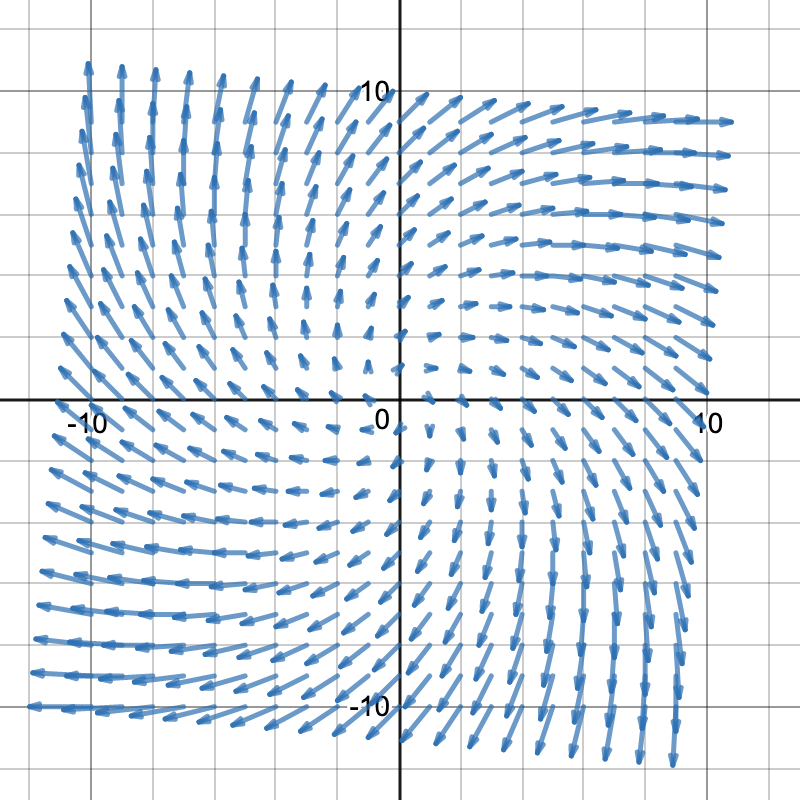
\includegraphics[width=.6\textwidth]{Figures/x+yx-y.png}
                \caption{The vector field $\mathbf{v}'(x,y)$ given by our system.}
                \label{fig:my_label}
            \end{figure}
            This solution has a stationary trajectory at the point $(0,0)$. Otherwise, the solution spirals outward in a clockwise direction. We say that this \emph{stationary point} $(0,0)$ is \emph{unstable}.
            \item Here is another example given by
            \begin{align*}
                x' &= -x +y,\\
                y' &= -x -y.
            \end{align*}
            Here is the plot of the vector field
            \begin{figure}[H]
                \centering
                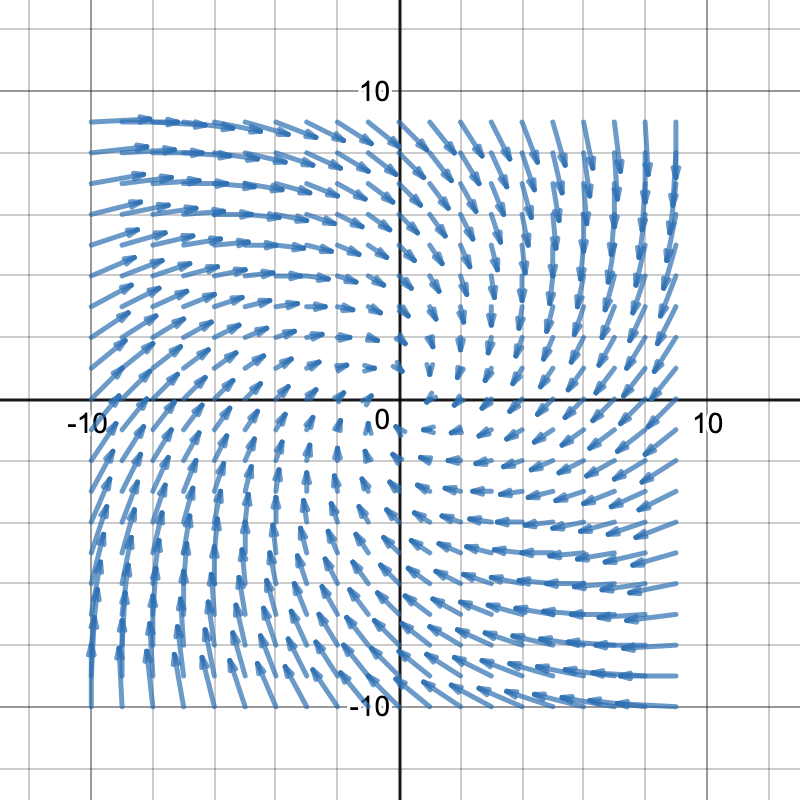
\includegraphics[width=.6\textwidth]{Figures/-x+y-x-y.png}
                \caption{The vector field $\mathbf{v}'(x,y)$ given by our system.}
                \label{fig:my_label}
            \end{figure}
            Here our solution again has a stationary trajectory at the point $(0,0)$.  Otherwise, the solution spirals inward in a clockwise direction.  Here we say that the stationary point $(0,0)$ is \emph{stable}.
            \item Let us take yet another example given by
            \begin{align*}
                x' &= y,\\
                y' &= -x.
            \end{align*}
            This has a vector field plot
            \begin{figure}[H]
                \centering
                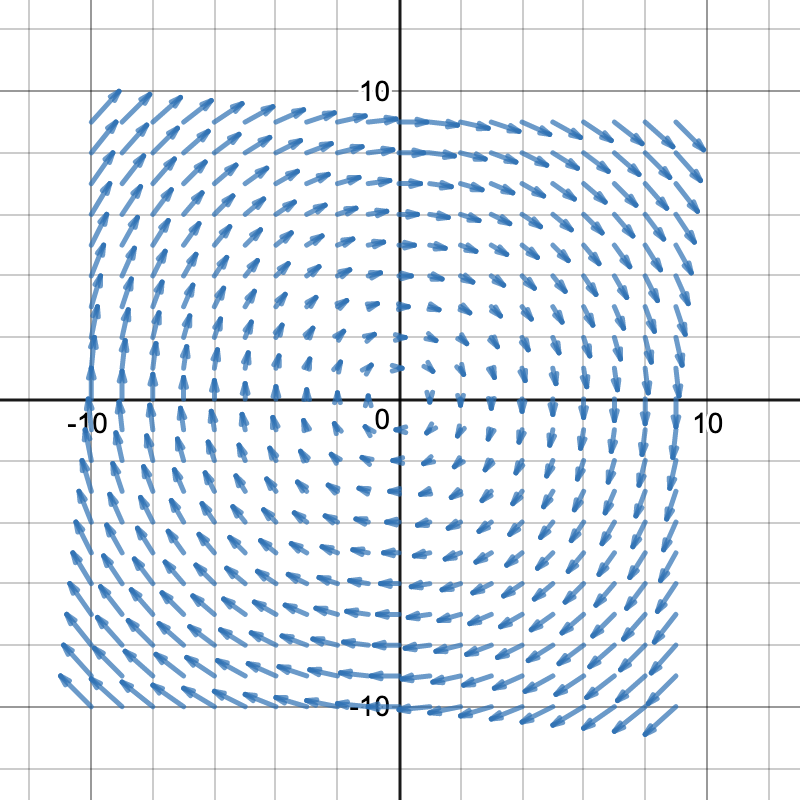
\includegraphics[width=.6\textwidth]{Figures/y-x.png}
                \caption{The vector field $\mathbf{v}'(x,y)$ given by our system.}
                \label{fig:my_label}
            \end{figure}
            Again, $(0,0)$ is a stationary point.  All the other trajectories form circles that rotate counter clockwise about the origin.
        \end{enumerate}
        \end{ex}
        
        These systems above show the four main dynamics we can see in the plane. All dynamics in the plane roughly look like one of these in close proximity to any point.
        
        \begin{ex}{General Solutions to the Zoo of Linear Systems}{gen_solns_zoo}
        We can look at the integral curves for these vector fields.  Without solving them explicitly, let's see what they would look like.
        \begin{enumerate}[(I)]
            \item The general solution for this system is
            \begin{align*}
                x(t)&= \frac{1}{2}c_1 \left( e^{2t}+1\right)+\frac{1}{2}c_2\left(e^{2t}-1\right),\\
                y(t)&=\frac{1}{2}c_1 \left( e^{2t}-1\right)+\frac{1}{2}c_2\left(e^{2t}+1\right).
            \end{align*}
            The initial data is dictated by the problem, and comes in the form of knowing $(x(0),y(0))$.  Here is a plot of a few integral curves (trajectories).
            \begin{figure}[H]
                \centering
                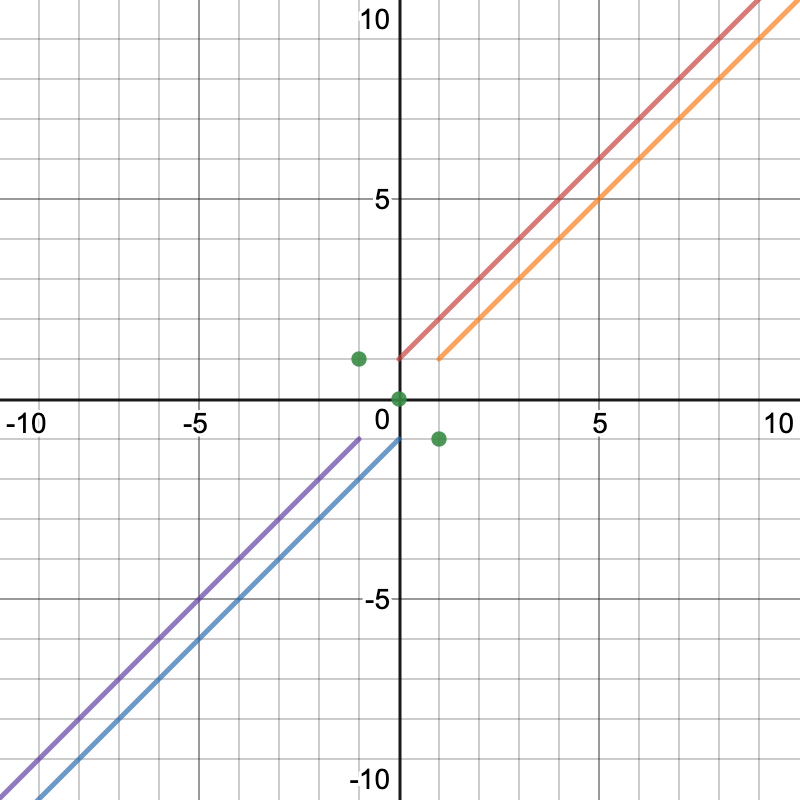
\includegraphics[width=.6\textwidth]{Figures/x+yx+yintegralcurves.png}
                \caption{Integral curves. Red: $(0,1)$; Orange: $(1,1)$; Purple: $(-1,-1)$; Blue: $(0,-1)$. Green are all stationary points.}
                \label{fig:my_label}
            \end{figure}
            \item The general solution for this system is
            \begin{align*}
                x(t)&= c_2 e^t \sin(t)+c_1e^t\cos(t),\\
                y(t)&= c_2 e^t \cos(t) - c_1e^1 \sin(t).
            \end{align*}
            Here are trajectories. Keep in mind these move radially \emph{outward} away from the stationary point!
                        \begin{figure}[H]
                \centering
                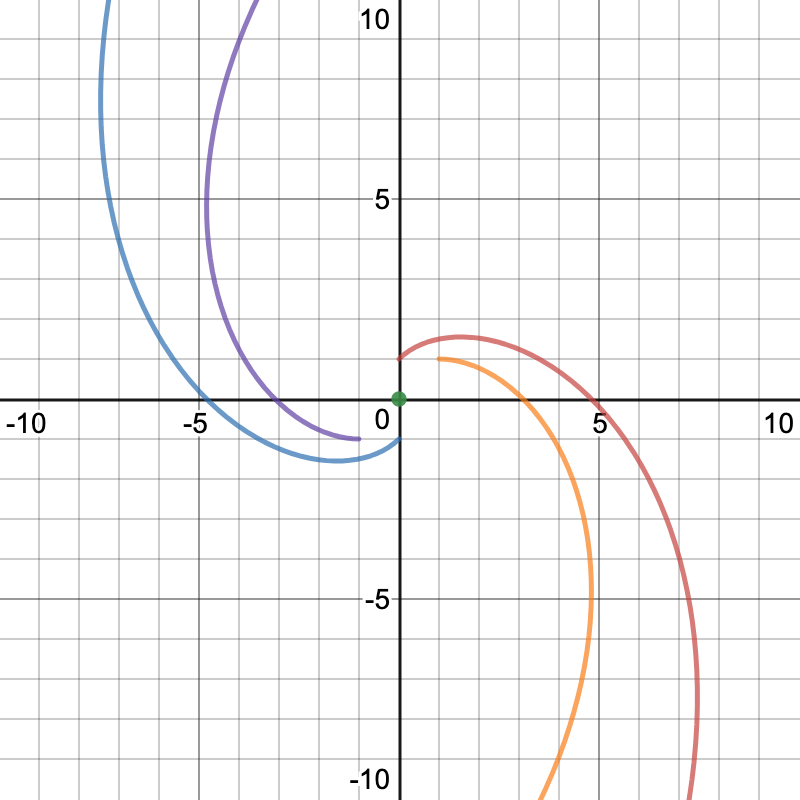
\includegraphics[width=.6\textwidth]{Figures/x+y-x+yintegralcurves.png}
                \caption{Integral curves. Red: $(0,1)$; Orange: $(1,1)$; Purple: $(-1,-1)$; Blue: $(0,-1)$. Green:$(0,0)$ is the stationary point.}
                \label{fig:my_label}
            \end{figure}
            \item The general solution for this system is
            \begin{align*}
                x(t)&=c_2 e^{-t}\sin(t)+c_1 e^{-t}\cos(t),\\
                y(t)&=c_2e^{-t}\cos(t)-c_1e^{-t}\sin(t).
            \end{align*}
            Here are trajectories. Keep in mind these are moving radially \emph{inward} towards the stationary point! Also note the difference in scale here.
            \begin{figure}[H]
                \centering
                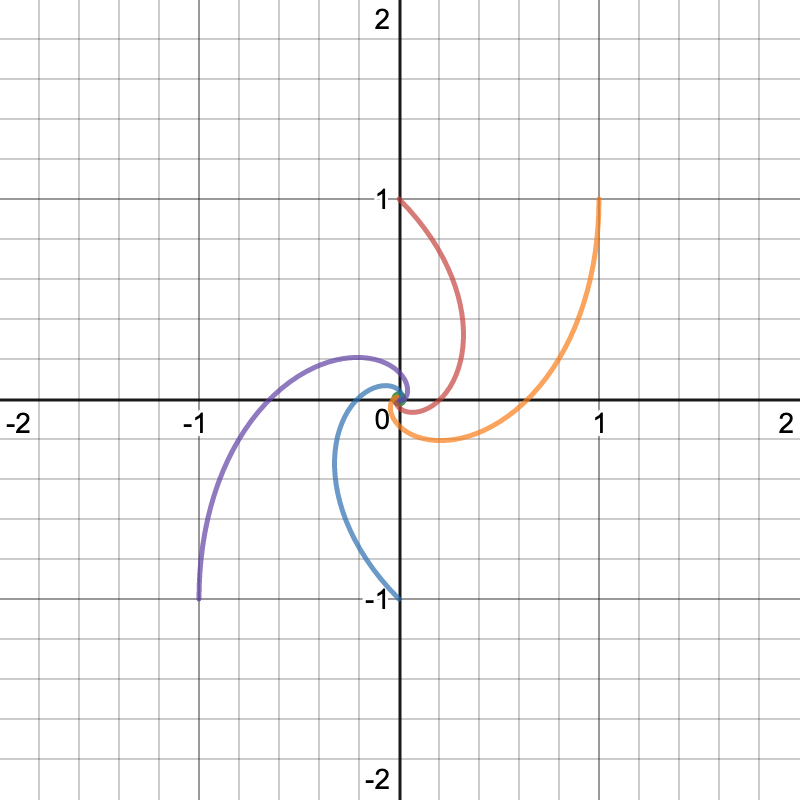
\includegraphics[width=.6\textwidth]{Figures/-x+y-x-yintegralcurves.png}
                \caption{Integral curves. Red: $(0,1)$; Orange: $(1,1)$; Purple: $(-1,-1)$; Blue: $(0,-1)$. Green: $(0,0)$ is the stationary point.}
                \label{fig:my_label}
            \end{figure}
            \item The general solution for this system is
            \begin{align*}
                x(t)&= c_2 \sin(t) + c_1 \cos(t),\\
                y(t)&= c_2 \cos(t) - c_1 \sin(t).
            \end{align*}
            Some of the trajectories here end up overlapping if we plot them over too much time.  Here's what I mean.
            \begin{figure}[H]
                \centering
                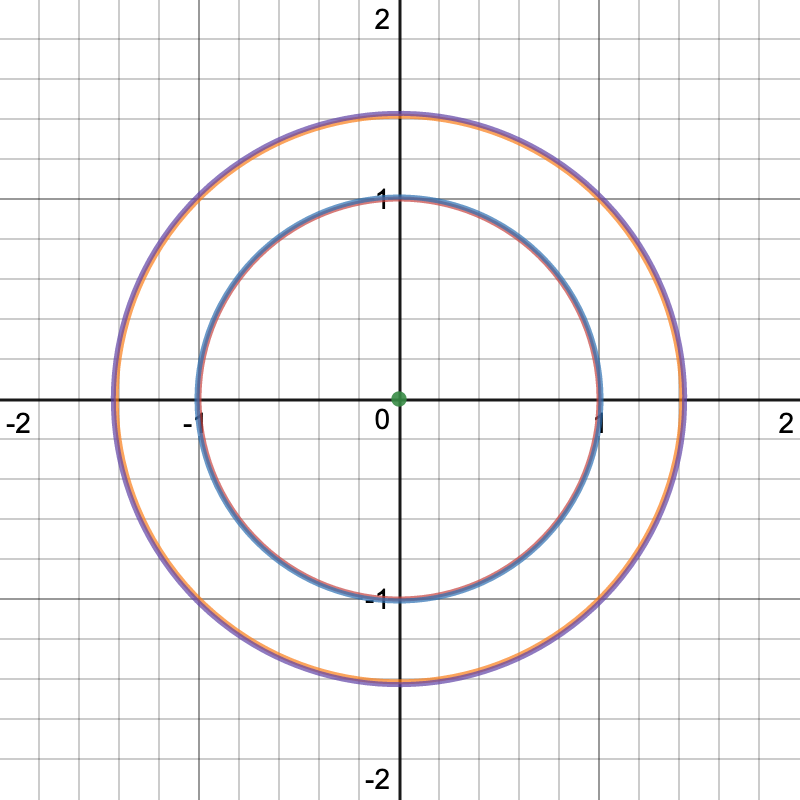
\includegraphics[width=.6\textwidth]{Figures/y-xintegralcurves.png}
                \caption{Integral curves. Red: $(0,1)$; Orange: $(1,1)$; Purple: $(-1,-1)$; Blue: $(0,-1)$. Green: $(0,0)$ is the stationary point.}
                \label{fig:my_label}
            \end{figure}
            However, here is what it looks like over a shorter period of time.
            \begin{figure}[H]
                \centering
                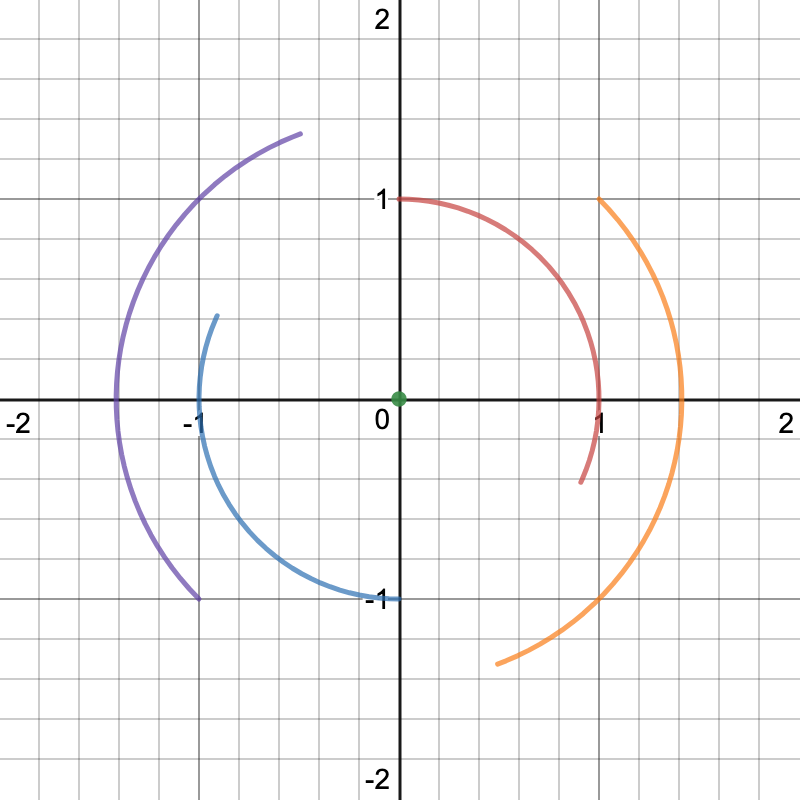
\includegraphics[width=.6\textwidth]{Figures/y-xintegralcurves2.png}
                \caption{Integral curves. Red: $(0,1)$; Orange: $(1,1)$; Purple: $(-1,-1)$; Blue: $(0,-1)$. Green: $(0,0)$ is the stationary point.}
                \label{fig:my_label}
            \end{figure}
            In a sense, each chosen initial conditions will chase one of the others forever in time.
        \end{enumerate}
        \end{ex}
        
        \section{Linearity}
        The above systems were all \emph{linear}.  These systems are in fact exactly solvable.  We'll get to the solutions shortly.  However, many systems in nature are \emph{nonlinear}.  Take for example, the SIR model. What does it mean for an ODE to be linear? 
        
        \begin{df}{Linear and Nonlinear ODE}{lin_ode}
        An $n$th order ODE is \textbf{linear} if it can take the following form
        \[
        x^{(n)}(t)+f_{n-1}(t)x^{(n-1)}(t)+\cdots + f_1(t)x'(t) +f_0(t)x(t)=g(t).
        \]
        This looks a bit complicated, so let's restate this for second order ODE.
        
        A second order $ODE$ is \textbf{linear} if it can take the following form
        \[
        x''+f(t)x'+g(t)x=h(t).
        \]
        And a first order ODE is linear if it can take the form
        \[
        x'+f(t)x=g(t).
        \]
        
        If an ODE does not satisfy the above definition, we say that it is \textbf{nonlinear}.
        \end{df}
        
        
        \section{Higher Order ODE}
        Higher order ODE show up in nature quite often.  For example, second order equations are abundant in physics due to Newton's laws.  Equations of order higher than two appear in material strain and stress (which tend to be fourth order).  
        
        The wonderful fact is that we do not need any new theory to understand higher order ODE.  This is due to the following theorem.
        
        \begin{thm}{Reduction of Order}{red_of_order}
        Any $n ^\textrm{th}$ order ODE is equivalent to a system of $n$ first order ODE.  
        \end{thm}
        
        The moral is that we need only know how to analyze first order systems in order to understand \emph{any} possible ODE.  Let's see an example of this.
        
        \begin{ex}{Order Reducing the Harmonic Oscillator}{order_red_harm_osc}
        Consider the harmonic oscillator equation
        \[
        x''=-x.
        \]
        We can define a new variable, $v$ so that $v=x'$.  Then note we have that $v'=x''$.  Substituting these gives us two first order equations
        \begin{align*}
            x'&=v,\\
            v'&=-x.
        \end{align*}
        It may seem like we have essentially done nothing.  But we've actually changed the problem for the better.  We'll see why soon.
        \end{ex}
        
        \begin{ex}{The Biharmonic Equation}{biharmonic_eq}
        Consider the \emph{biharmonic equation}
        \[
        x''''=x.
        \]
        We can define a set of new variables $y=x'$, $z=y'$, and $w=z'$.  Note that $w'=z''=y'''=x''''$. Then we arrive at the system
        \begin{align*}
            x'&=y,\\
            y'&=z,\\
            z'&=w,\\
            w'&=x.
        \end{align*}
        We have turned a fourth order ODE into a system of four first order ODE.
        \end{ex}
        
        \section{Linear Systems}
        Let's say we are given a nonlinear higher order ODE or system. We wish to be able to convert this to a linear problem of the form 
        \[
        \mathbf{v}'=A\mathbf{v}+\mathbf{F}
        \]
        where, for example, 
        \[
        \mathbf{v}=\begin{bmatrix} x(t) \\ y(t) \\ z(t) \end{bmatrix} \qquad \mathbf{v}'=\begin{bmatrix} x'(t) \\ y'(t) \\ z'(t) \end{bmatrix} \qquad \begin{bmatrix} f_1(t) \\ f_2(t) \\ f_3(t) \end{bmatrix}.
        \]
        We call this the \emph{inhomogeneous} system. 
        
        Roughly speaking, we can think of $\mathbf{F}$ as an external forcing term acting on the system.  We will concentrate more on solving the case where $\mathbf{F}=\mathbf{0}$ so that we have
        \[
        \mathbf{v}'=A\mathbf{v}.
        \]
        We call this the \emph{homogeneous} system. Here, $A$ is a $3\times 3$-matrix whose coefficients could possibly depend on time.  That is,
        \[
        A = \begin{bmatrix} A_{11}(t) & A_{12}(t) & A_{13}(t)\\
        A_{21}(t) & A_{22}(t) & A_{23}(t)\\
        A_{31}(t) & A_{32}(t) & A_{33}(t)\end{bmatrix}.
        \]
        We will ignore the case where the matrix depends on time and just work on the case where the coefficients are constant. This is called an \emph{autonomous} system.
        
        \begin{df}{Linear System of ODE}{linear_system}
            A system of first order differential equations is \textbf{linear} if it can be expressed as a matrix equation
            \[
            \mathbf{v}' = A(t)\mathbf{v}+\mathbf{F}(t).
            \]
            The linear system is said to have \textbf{constant coefficients} if the matrix $A(t)$ only contains constant.  That is, $A$ does not actually depend on $t$.
        \end{df}
        
        \begin{df}{Homogeneous and Inhomogeneous Linear Systems}{homogeneous_systems}
            A linear system of differential equations is 
            \textbf{inhomogeneous} if it can be expressed as
            \[
            \mathbf{v}' = A(t)\mathbf{v}+\mathbf{F}(t).
            \]
            If $\mathbf{F}(t)=0$ and we have
            \[
            \mathbf{v}' = A(t)\mathbf{v}
            \]
            then we say the system of differential equations is \textbf{homogeneous}.
        \end{df}
        
        \begin{df}{Autonomous}{autonomous}
        An \textbf{autonomous} first order system (in 3-dimensions) is given by the equations
        \begin{align*}
        x' &= f(x,y,z),\\
        y' &= g(x,y,z),\\
        z' &= h(x,y,z).
        \end{align*}
        This is autonomous due to the fact that $t$ does not appear as an argument for the functions $f,g,$ and $h$.
        \end{df}
        
        Autonomous systems are extremely common in reality which is why it is not a bad idea to emphasize them here.  These are the systems in which some quantity is being conserved over time, and hence the apparent $t$ dependence of the functions (shown above) is gone.  Of course, the functions still depend on $t$!  A few examples are
        \begin{itemize}
            \item mechanical systems (energy is conserved),
            \item closed thermodynamic systems (energy is conserved),
            \item short time ecologocial systems (animal number is conserved), 
            \item closed chemically reacting systems (total atomic count is constant).
        \end{itemize}
        
        For us, we are going to concentrate on dynamics for a system of two equations.  That is, equations that exist in the plane.  For one, these systems are easier to solve by hand than the higher dimensional systems.  They are also very common to see due again to Newton's laws.  Often, we will find we can decompose larger systems of equations into sets of systems of two equations. Lastly, these are likely the easiest to visualize and build intuition with.  
        
        \section{Linearization}
        If we are given a planar (autonomous) and possibly nonlinear system, 
        \begin{align*}
            x'&= f(x,y),\\
            y'&= g(x,y),
        \end{align*}
        we want to approximate this system with a homogeneous linear system with a matrix with constant coefficients.  That is
        \[
        \begin{bmatrix} x' \\ y' \end{bmatrix} \approx \begin{bmatrix} A_{11} & A_{12} \\ A_{21} & A_{22} \end{bmatrix} \begin{bmatrix} x \\ y \end{bmatrix}.
        \]
    
        Remember that what we have here is a 2-dimensional vector field given by our system
        \[
        \mathbf{v}(x,y) = \begin{bmatrix} f(x,y) \\ g(x,y) \end{bmatrix}.
        \]
        The best linear approximation to this vector field at a point $(x_0,y_0)$ is given by the Jacobian $J(x_0,y_0)$ for this vector field
        \[
        J(x_0,y_0) = \begin{bmatrix} \frac{\partial f}{\partial x}(x_0,y_0) & \frac{\partial f}{\partial y}(x_0,y_0) \\
        \frac{\partial g}{\partial x}(x_0,y_0) & \frac{\partial g}{\partial y}(x_0,y_0) \end{bmatrix}.
        \]
        We will then let the coefficient matrix be given by this Jacobian.  That is, we get
        \[
        \begin{bmatrix} x' \\ y' \end{bmatrix} = J(x_0,y_0)\begin{bmatrix} x \\ y \end{bmatrix}.
        \]
        Let's work an example.
        
        \begin{ex}{Lotka-Volterra Model Linearization}{lotka_volterra_linearization}
        Let us consider a predator and prey system given by the Lotka-Volterra model.  Here we let the number of prey be given by $R(t)$ and the number of predators be given by $S(t)$.  The system is
        \begin{align*}
            S' &= (-c+dR)S,\\
            R' &= (a-bS)R,
        \end{align*}
        where $a,b,c,d>0$. Here we can say that we have
        \begin{align*}
        f(S,R) &= (-c+dR)S,\\
        g(S,R) &= (a-bS)R.
        \end{align*}
        We compute each partial derivative
        \begin{align*}
            \frac{\partial f}{\partial S} &= -c+dR & \frac{\partial f}{\partial R} &=dS \\
            \frac{\partial g}{\partial S} &= -bR & \frac{\partial g}{\partial R} &= a-bS.
        \end{align*}
        Evaluating each at the point $(S_0,R_0)$ and placing into a matrix gives us the Jacobian
        \[
        J(S_0,R_0)=\begin{bmatrix} -c+dR_0 & dS_0 \\ -bR_0 & a-bS_0 \end{bmatrix}.
        \]
        
        Now, about this point, our system approximately takes the form
        \[
        \begin{bmatrix} S' \\ R' \end{bmatrix} = \begin{bmatrix} -c+dR_0 & dS_0 \\ -bR_0 & a-bS_0 \end{bmatrix} \begin{bmatrix} S \\ R \end{bmatrix}.
        \]
        \end{ex}
        
        Our goal now is to learn how we can explicitly solve these planar systems.  With that, we will be able to solve many problems.
        
        
        Now that we can take many common ODE, convert them to a system of first order ODE, and linearize the system, we can work to solve these specific equations.  The detail is captured by the following.
        
        \begin{prop}{Eigenfunction of the Derivative}{eigenfunction}
        The exponential function $e^{kx}$ is an \textbf{eigenfunction} for the derivative.  \\
        
        \noindent \emph{Proof.} We take 
        \[
        \frac{d}{dt} e^{kt} = ke^{kt}.
        \]
        So, the eigenvalue is $k$ for this eigenfunction. \qed
        \end{prop}
        
        
        Spending the time being more rigorous with this is an interesting endeavor, but we have done enough theoretical results for now.  Let us see an example.
        
        \begin{ex}{Harmonic Oscillator Eigenvalue}{harm_osc_eigen}
        If we take the Harmonic Oscillator equation
        \[
        x'' = -x
        \]
        we can realize this extremely similar to an eigen equation with
        \[
        x'=ix.
        \]
        So, this eigen equation has a solution
        \[
        x(t)=e^{it}.
        \]
        Note that this solves the Harmonic oscillator equation since
        \[
        \frac{d^2}{dt^2} x(t) = \frac{d}{dt}ie^{it} = -e^{it}=-x.
        \]
        Remember that
        \[
        e^{it}=\cos(t)+i\sin(t)
        \]
        which captures the oscillating behavior.
        \end{ex}
        
        In short, these exponential functions capture oscillations, growth, and decay.  With these functions, we can model all linear systems.
        
        \begin{prop}{General Solution to Planar Linear Systems}{gen_soln_lin_systems}
        Given a two dimensional linear system with constant coefficients $A,B,C$, and $D$,
        \begin{align*}
        x' &= Ax+By,\\
        y' &= Cx+Dy,
        \end{align*}
        we can write this as a matrix equation
        \[
        \begin{bmatrix} x' \\ y' \end{bmatrix} = \begin{bmatrix} A & B\\ C & D \end{bmatrix} \begin{bmatrix} x \\ y \end{bmatrix},
        \]
        with
        \[
        M=\begin{bmatrix} A & B \\ C & D \end{bmatrix}.
        \]
        Let $\lambda_1$ and $\lambda_2$ be the (complex) eigenvalues of $M$ and $\mathbf{v}_1$ and $\mathbf{v}_2$ be the corresponding eigenvectors.  Then, the solution to the system of equations is
        \[
        \begin{bmatrix} x(t) \\ y(t) \end{bmatrix} = c_1 \mathbf{v}_1 e^{\lambda_1t} + c_2 \mathbf{v}_2e^{\lambda_2 t}.
        \]
        \end{prop}
        
        Let us unravel this with an example problem.
        
        \begin{ex}{Damped Harmonic Motion}{damped_harm_motion}
        Consider the Damped Harmonic Oscillator equation
        \[
        x'' +\mu x' + kx = 0,
        \]
        with initial data $x(0)=1$ and $x'(0)=0$.\\ 
        
        Let us first think about this problem with our intuition.  This equation is modelling a spring mass system that is in a damping medium (i.e., underwater).  What happens as this system evolves?  One should expect oscillation, but will the system oscillate indefinitely? No.  One should expect that this system will also begin to oscillate with less intensity over time.  With this, one could hazard a guess that
        \[
        x(t) \approx e^{-t}\cos(t).
        \]
        
        We can reduce the order of this equation by letting $y=x'$.  This gives us the system
        \begin{align*}
        x' &= y,\\
        y' &= -kx -\mu y.
        \end{align*}
        So we can write this as a matrix equation
        \[
        \begin{bmatrix} x' \\ y' \end{bmatrix} = \begin{bmatrix} 0 & 1 \\ -k & -\mu \end{bmatrix}.
        \]
        For simplicity, let $k=\mu=1$, and we get the matrix
        \[
        M = \begin{bmatrix} 0 & 1 \\ - 1& - 1 \end{bmatrix}.
        \]
        Then the eigenvalues to this matrix are
        \[
        \lambda_1 = \frac{1}{2}(-1+i\sqrt{3})\quad \textrm{and} \quad \lambda_2 = \frac{1}{2}(-1-i\sqrt{3}).
        \]
        The eigenvectors are
        \[
        \mathbf{v}_1 = \begin{bmatrix} \frac{1}{2} (-1-i\sqrt{3}) \\ 1 \end{bmatrix} \quad \textrm{and} \quad \mathbf{v}_2 = \begin{bmatrix} \frac{1}{2} (-1+i\sqrt{3}) \\ 1 \end{bmatrix}.
        \]
        By the proposition, our solution is
        \[
        \begin{bmatrix} x(t) \\ y(t) \end{bmatrix} = c_1 \begin{bmatrix} \frac{1}{2} (-1-i\sqrt{3}) \\ 1 \end{bmatrix} e^{\frac{1}{2}(-1+i\sqrt{3})t}+c_2  \begin{bmatrix} \frac{1}{2} (-1+i\sqrt{3}) \\ 1 \end{bmatrix} e^{\frac{1}{2}(-1-i\sqrt{3})t}.
        \]
        However, in this case we are wishing to just find $x(t)$ that fits this data, and what we find is this system of equations reduces to
        \begin{align*}
        x(t) &= c_1 e^{\frac{1}{2}(-1+i\sqrt{3})t}+c_2 e^{\frac{1}{2}(-1-i\sqrt{3})t},
        \end{align*}
        by looking at just the first entry of each vector and realizing that since $c_1$ and $c_2$ are undetermined constants, we can remove the other constants that appear.
        
        Now, let's use Euler's formula, and we have
        \begin{align*}
            x(t) &= c_1 e^{\frac{1}{2}(-1+i\sqrt{3})t}+c_2 e^{\frac{1}{2}(-1-i\sqrt{3})t}\\
            &= c_1 e^{-t/2}\left(\cos\left(\frac{\sqrt{3}}{2}t\right)+i\sin\left(\frac{\sqrt{3}}{2}t\right)\right)+c_2 e^{-t/2}\left(\cos\left(-\frac{\sqrt{3}}{2}t\right)+i\sin\left(-\frac{\sqrt{3}}{2}t\right)\right).
        \end{align*}
        There are a few more simplifications that can be done, but in the end we find the general solution
        \[
        x(t) = c_1 e^{-t/2} \sin\left(\frac{\sqrt{3}}{2}t\right)+c_2e^{-t/2}\cos\left(\frac{\sqrt{3}}{2}t\right).
        \]
        We were given that $x(0)=1$ and we have that
        \[
        x(0)=1=c_2
        \]
        by plugging into our general solution.  We also have that
        \[
        x'(0)=0=\frac{-\sqrt{3}}{4}c_1
        \]
        which means $c_1=0$.  So our particular solution is
        \[
        x_p(t) = e^{-1/2t}\cos \left(\frac{\sqrt{3}}{2}t\right).
        \]
        
        This solution also seems fit our physical expectations of the damped spring-mass system.  Great!
        \end{ex}
        
        \begin{exercise}
        Verify that this $x_p$ above is indeed a solution to the original ODE with $k=\mu=1$.
        \end{exercise}

        \begin{remark}
        The apparent difficulty of solving ODEs becomes obvious here.  In this extremely nice case it still took a large amount of work.  The case for other systems is generally worse.
        \end{remark}
        
        \section{General Solutions to Second Order Linear Equations}
        
        We can now write the general solutions to all second order linear equations.  We have the following.
        
        \begin{prop}{General Solutions to Second Order Linear Equations}{gen_solns_second_order}
        Given a second order homogeneous linear ODE
        \[
        x'' + \mu x' + kx = 0
        \]
        we can write this as a system of first order linear equations given by
        \[
        \mathbf{v}' = M \mathbf{v},
        \]
        where
        \[
        \mathbf{v} = \begin{bmatrix} x \\ y \end{bmatrix}.
        \]
        the eigenvalues of $M$ are either purely real or complex.
        
        \begin{itemize}
            \item If the eigenvalues $\lambda_1$ and $\lambda_2$ are complex, then the solution is
        \[
        x(t)= c_1 e^{\RE(\lambda_1)t} \sin(\IM(\lambda_1)t) + c_2 e^{\RE(\lambda_1)t} \sin(\IM(\lambda_1)t).
        \]
        It does not actually matter if we choose $\lambda_1$ or $\lambda_2$!
        \item         If the eigenvalues $\lambda_1$ and $\lambda_2$ are real then the general solution is:
        \[
        x(t) = c_1 e^{\lambda_1 t} + c_2 e^{\lambda_2 t}.
        \]
        \end{itemize}
        \end{prop}
        
        
% %%%%%%%%%%%%%%%%%%%%%%%%%%%%%%%%%%%%%%%%%%%%%%%%%%%%%%%%%%%%%%%%%%%%%%%%%%%%%%%%%%%%
% Partial Differential Equations
% %%%%%%%%%%%%%%%%%%%%%%%%%%%%%%%%%%%%%%%%%%%%%%%%%%%%%%%%%%%%%%%%%%%%%%%%%%%%%%%%%%%%
        
        \chapter{Partial Differential Equations}
        
        We now want to investigate a larger class of differential equations.  These are the \emph{partial differential equations} or PDE.  These equations become yet more complicated to solve, but are very prevalent in the study of the physical world.
        
        Fundamentally, these are time-varying differential equations of vector and scalar fields of many variables.  The goal for us is to be able to recognize a few specific example equations and understand their behavior.  We will also be able to solve a few equations with our tools from studying ODE. However, it is easy to pose a PDE that is virtually impossible to solve.  
        
        \begin{df}{Partial Differential Equation}{pde}
        A \textbf{partial differential equation of a scalar field} of three spatial variables $x,y,z$ and a time variable $t$ is an expression of a scalar function $u(x,y,z,t)$, the partial derivatives of $u(x,y,z,t)$, and other functions.
        \end{df}
        
        \begin{df}{Vector Partial Differential Equation}{vec_pde}
        A \textbf{partial differential equation of a vector field}
        \[
        \mathbf{v}(x,y,z,t) = \begin{bmatrix} v_1(x,y,z,t) \\ v_2(x,y,z,t) \\ v_3(x,y,z,t) \end{bmatrix}
        \]
        is an equation containing $\mathbf{v}$, the (component) derivatives of $\mathbf{v}$, and other vector fields.
        \end{df}
        
        With the difficulty of these expressions as is, we will concentrate solely on the equations with scalar functions.
    % %%%%%%%%%%%%%%%%%%%%%%%%%%%%%%%%%%%%%%%%%%%%%%%%%%%%%%%%%%%%%%%%%%%%%%%%%%%%%%%%%%%%
    % Examples of PDE
    % %%%%%%%%%%%%%%%%%%%%%%%%%%%%%%%%%%%%%%%%%%%%%%%%%%%%%%%%%%%%%%%%%%%%%%%%%%%%%%%%%%%%
    
        \section{Examples of PDE}
        
        \begin{ex}{Heat Equation}{heat_eqn}
        The \textbf{heat equation} in three dimensional space is the equation
        \[
        \frac{\partial u}{\partial t}(x,y,z,t) -k\nabla \cdot (\nabla u(x,y,z,t)) = f(x,y,z,t).
        \]
        This equation models the diffusion of heat in a region of space, hence the name.  In this case, we think of $u(x,y,z,t)$ being the temperature at the point $(x,y,z)$ at the time $t$.
        \end{ex}
        
        \begin{ex}{Laplace (Poisson) Equation}{laplace}
        The \textbf{Laplace} (sometimes \textbf{Poisson}) \textbf{equation} in three dimensional space is the equation
        \[
        -\nabla \cdot (\nabla u(x,y,z))=f(x,y,z).
        \]
        \emph{Notice, there is no dependence on time!} This equation is the long term behavior of the heat equation.  If $u(x,y,z)$ describes temperature, then the solution to this equation tells you the equilibrium temperature. Since this is an equilibrium solution, the time component is gone.
        \end{ex}
        
        \begin{ex}{The Wave Equation}{wave}
        The \textbf{wave equation} in three dimensional space is the equation
        \[
        \frac{\partial^2 u}{\partial^2 t}(x,y,z,t) -c^2\nabla \cdot (\nabla u(x,y,z,t)) = f(x,y,z,t).
        \]
        The solutions here are wavelike.  Think of plucking a guitar string, or the ripples on the surface of a lake after a rock has been tossed in, or the vibrating cymbal or drum head.
        \end{ex}
        
        \begin{ex}{Maxwell's Equations}{maxwell}
        Maxwell's equations describe the electric $\mathbf{E}$ and magnetic $\mathbf{B}$ fields that permeate space due to charged particles.  These equations turn out to be coupled PDE.  They read
        \begin{align*}
            \nabla \cdot \mathbf{E}(x,y,z,t) &= \frac{\rho(x,y,z,t)}{\epsilon},\\
            \nabla \cdot \mathbf{B}(x,y,z,t) &= 0,\\
            \nabla \times \mathbf{E}(x,y,z,t) &= -\frac{\partial B}{\partial t}(x,y,z,t),\\
            \nabla \times \mathbf{B}(x,y,z,t) &= \mu \mathbf{J} + \mu \epsilon \frac{\partial \mathbf{E}}{\partial t}(x,y,z,t).
        \end{align*}
        \end{ex}
        
        \section{The Problem Statement}
        
        In order to move forward, we need to also properly specify the problem we want to solve.
        
        The one-dimensional source-free heat equation is a great starting point to begin our process.  We are given the following data:
        \begin{itemize}
            \item A region $\Omega$ in space that we are concerned with.  For example, in one dimension, we can consider the interval $\Omega=(0,1)$.
            \item A PDE
            \[
            \frac{\partial u}{\partial t}(x,t) -k \frac{\partial^2 u}{\partial x}^2 = 0.
            \]
            \item Boundary conditions. These can come in a few forms, but we will concentrate on just one. We must specify $u(0,t)=a$ and $u(1,t)=b$.  These boundary conditions correspond to fixing the temperature at the ends of a rod constant.
            \item Initial conditions. We specify the initial temperature distribution
            \[
            u(x,0)=u_0(x).
            \]
        \end{itemize}
    
    % %%%%%%%%%%%%%%%%%%%%%%%%%%%%%%%%%%%%%%%%%%%%%%%%%%%%%%%%%%%%%%%%%%%%%%%%%%%%%%%%%%%%
    % The Heat Equation
    % %%%%%%%%%%%%%%%%%%%%%%%%%%%%%%%%%%%%%%%%%%%%%%%%%%%%%%%%%%%%%%%%%%%%%%%%%%%%%%%%%%%%
    
        \section{The Heat Equation}
        One of the most illuminating examples of PDEs is the \emph{heat equation}.  Let us work through a specific example of the heat equation and keep in mind the physical intuition throughout.
        
        \begin{ex}{Solving the Heat Equation}{solving_heat_equation}
        Let us consider the simplified one-dimensional source free heat equation given by the following:
        \[
        \frac{\partial u}{\partial t}(x,t)-\frac{\partial^2 u}{\partial x^2} = 0.
        \]
        We can require boundary conditions and initial conditions later on.\\
        
        Let us assume that the solution function $u(x,t)$ can be written as
        \[
        u(x,t) = f(x)g(t).
        \]
        We call this approach the \textbf{separation of variables}. We then plug in this assumption to our PDE.
        \begin{align*}
            \frac{\partial}{\partial t} (f(x)g(t))-\frac{\partial^2}{\partial x^2} (f(x)g(t)) &= 0\\
            f(x)\frac{\partial g}{\partial t}-g(t)\frac{\partial^2 f}{\partial x^2}&=0\\
            fg'-f''g &=0.
        \end{align*}
        We can then do a bit more algebra.
        \begin{align*}
            fg'-f''g&=0\\
            fg'&= f''g\\
            \frac{g'(t)}{g(t)}&=\frac{f''(x)}{f(x)}.
        \end{align*}
        Now, notice that both sides depend on different variables.  We have successfully separated this equation into an equation for each variable.  This is to say, since each side of the equation depends on a different variable, each side must be equal to a constant $\lambda$! So we have two equations.
        \begin{align*}
            \frac{g'(t)}{g(t)}&=\lambda\\
            \frac{f''(x)}{f(x)}&=\lambda.
        \end{align*}
        We can then solve both of these as ODE. Note, it will be helpful to to instead choose $-\lambda$ as the constant.
        \end{ex}
        
        \begin{exercise}
        What are the general solutions to the above ODE?
        \end{exercise}
        
        \begin{exercise}
        Given those general solutions, what is the general solution to the heat equation?
        \end{exercise}
        
        \begin{answer}
        We get
        \[
        \boxed{u(x,t)=f(x)g(t) = Ae^{-\lambda t}\sin(\sqrt{\lambda}t)+Be^{-\lambda t}\cos(\sqrt{\lambda}t).}
        \]
        \end{answer}
        
        Previously we found the general solution to the heat equation 
        \[
        \frac{\partial u}{\partial t}(x,t) - \frac{\partial^2 u}{\partial x^2} (x,t) = 0
        \]
        is
        \[
        u(x,t)=Ae^{-\lambda t}\sin(\sqrt{\lambda}x)+Be^{-\lambda t}\cos(\sqrt{\lambda}x).
        \]
        However, this solution is very general.  We have the undetermined constants $\lambda$, $A$, and $B$. We need more information to get a particular solution.
        
        \begin{ex}{Particular Solution to the 1D Heat Equation}{particular_heat}
        We will stick with the one-dimensional case but we must pick the following.  
        \begin{itemize}
            \item Domain: Let $\Omega = (0,1)$.
            \item Initial Conditions: $u(x,0)=\sin(\pi x)$.
            \item Boundary Conditions: $u(1,t)=u(0,t)=0$.  
        \end{itemize}
        This list of requirements gives us enough information to solve the equation explicitly for a particular solution.\\
        
        First, let us take the boundary conditions. We impose these on our general solution:
        \[
        u(x,t)=Ae^{-\lambda t}\sin(\sqrt{\lambda}x)+Be^{-\lambda t}\cos(\sqrt{\lambda}x).
        \]
        Thus we require
        \[
        0=u(0,t)=Ae^{-\lambda t}\sin(0)+Be^{-\lambda t}\cos(0)
        \]
        which gives us that
        \[
        B=0.
        \]
        The other boundary condition is
        \[
        0=u(1,t)=Ae^{-\lambda t}\sin(\sqrt{\lambda}).
        \]
        Specifically, this means that $A=0$, which gives us a trivial solution or that we have
        \[
        \sqrt{\lambda}=n\pi
        \]
        for any integer $n$.  This is because $\sin(n\pi)=0$ when $n$ is an integer. Thus our solution now reads
        \[
        u(x,t)=Ae^{-n^2\pi^2}\sin(n\pi x).
        \]
        
        Lastly, we match our initial conditions.  So we have
        \[
        \sin(\pi x)=u(x,0)=A e^0 \sin(n\pi x)
        \]
        and so we find that $n=1$.  Thus, our solution is
        \[
        \boxed{u(x,t)=e^{-\pi^2 t} \sin(\pi x).}
        \]
        \end{ex}
        
        \begin{exercise}
        Can you interpret what this is physically describing as $t$ gets larger?
        \end{exercise}
        
    % %%%%%%%%%%%%%%%%%%%%%%%%%%%%%%%%%%%%%%%%%%%%%%%%%%%%%%%%%%%%%%%%%%%%%%%%%%%%%%%%%%%%
    % The Laplace Equation
    % %%%%%%%%%%%%%%%%%%%%%%%%%%%%%%%%%%%%%%%%%%%%%%%%%%%%%%%%%%%%%%%%%%%%%%%%%%%%%%%%%%%%
    
        \section{The Laplace Equation}
        In the long time limit ($t\to \infty$) or steady-state of the heat equation, one arrives at the so called Laplace equation
        \[
        -\nabla \cdot \nabla u = 0.
        \]
        In the one-dimensional case, this equation reads
        \[
        -\frac{d^2 u}{dx^2}(x) = 0.
        \]
        Note there is no dependence on time as this is the steady-state behavior for the heat equation.
        
        \begin{exercise}
        This is an ODE in the variable $x$.  You can solve this and find a general solution by integration.  
        \end{exercise} 
        
        \begin{answer}
        The general solution to the one-dimensional Laplace equation is the equation for a line
        \[
        u(x) = Ax+B.
        \]
        One can show that this is indeed a solution by taking two derivatives of $u(x)$ and finding that you get zero.
        \end{answer}
        
        \begin{ex}{Particular Solution to the 1D Laplace Equation}{particular_laplace}
        Through integration, we find
        \[
        u(x) = Ax+B
        \]
        where $A$ and $B$ are undetermined constants.  In order to specify these constants, we must provide the following.
        \begin{itemize}
            \item Domain: Let $\Omega = (0,1)$.
            \item Boundary Conditions: $u(0)=0$ and $u(1)=0$.  
        \end{itemize}
        Note that we do not need initial conditions since there is no time dependence in this PDE.\\
        
        Now, to find the particular solution, we apply the boundary conditions to our general solution.  So we have
        \[
        0=u(0)=A(0)+B,
        \]
        so $B=0$.  Then the other condition 
        \[
        0=u(1)=A,
        \]
        so $A=0$.  Thus, our solution is
        \[
        \boxed{u(x)=0}.
        \]
        Now, compare this to the solution to the heat equation previously
        \[
        u(x,t)=e^{-\pi^2 t}\sin(\pi x).
        \]
        We claimed the Laplace equation is the long-time solution of the heat equation and indeed if we look at $t\to\infty$, we have
        \[
        \lim_{t\to \infty} u(x,t)=0.
        \]
        \end{ex}
        
    % %%%%%%%%%%%%%%%%%%%%%%%%%%%%%%%%%%%%%%%%%%%%%%%%%%%%%%%%%%%%%%%%%%%%%%%%%%%%%%%%%%%%
    % The Wave Equation
    % %%%%%%%%%%%%%%%%%%%%%%%%%%%%%%%%%%%%%%%%%%%%%%%%%%%%%%%%%%%%%%%%%%%%%%%%%%%%%%%%%%%%

        \section{The Wave Equation}
        The wave equation is studied when one wants to find the oscillatory behavior of some medium.  For example, one can pluck a guitar string or hit a drum head.  These actions induce vibrations in the medium (the string or head) and it is the vibrations that one hears.  The equation that models these phenomenon is the wave equation
        \[
        \frac{\partial^2 u}{\partial t^2}(x,y,z,t)-c^2 \nabla \cdot \nabla u(x,y,z,t)=f(x,y,z,t).
        \]
        
        \begin{ex}{Solving the 1D Wave Equation}{1d_wave}
        In one-dimension, the simplified source free wave equation reads
        \[
        \frac{\partial^2 u}{\partial t^2}(x,t) -\frac{\partial^2 u}{\partial x^2}(x,t)=0.
        \]
        
        It turns out we can solve the 1D wave equation in the same way we did the heat equation. So, we assume a separation of variables approach in that 
        \[
        u(x,t) = f(x)g(t).
        \]
        We plug this into the PDE to find
        \begin{align*}
            \frac{\partial^2}{\partial t^2}(f(x)g(t))-\frac{\partial^2}{\partial x^2}(f(x)g(t))&=0\\
            f(x)\frac{\partial^2 g}{\partial t^2}-g(t)\frac{\partial^2 f}{\partial x^2}&=0\\
            f(x)g''(t)-f''(x)g(t)&=0.
        \end{align*}
        We then wish to make the left hand side and right hand side functions of different input variables
        \begin{align*}
            f(x)g''(t)-f''(x)g(t)&=0\\
            f(x)g''(t)&=f''(x)g(t)\\
            \frac{g''(t)}{g(t)}&= \frac{f''(x)}{f(x)}.
        \end{align*}
        Since each side depends on a different input variable, each side must be equal to a constant.  So this gives us
        \[
        \frac{g''(t)}{g(t)}= \frac{f''(x)}{f(x)}= -\lambda^2,
        \]
        where $-\lambda^2$ is an undetermined constant but was chosen to make the next steps easier. We then get two ODEs
        \begin{align*}
            f''(x)&=-\lambda^2 f(x),\\
            g''(t)&=-\lambda^2 g(t),
        \end{align*}
        which are both harmonic oscillator equations.  Thus, since we know the solutions to the harmonic oscillator equation, we have
        \begin{align*}
            f(x)&=C_1 \sin(\lambda x)+ C_2 \cos(\lambda x),\\
            g(t)&=C_3 \sin(\lambda t)+ C_3 \cos(\lambda t).
        \end{align*}
        It follows that our solution is thus
        \[
        \boxed{u(x,t)=f(x)g(t)= (C_1 \sin(\lambda x)+ C_2 \cos(\lambda x))(C_3 \sin(\lambda t)+ C_3 \cos(\lambda t)).}
        \]
        \end{ex}
        
        With a general solution to the wave equation written down.  We can work to solve a particular case of the wave equation.  Let's see this.
        
        \begin{ex}{Particular Solution to the 1D Wave Equation}{part_wave}
        We found that the general solution to the 1D wave equation is
        \[
        u(x,t)=(C_1 \sin(\lambda x)+ C_2 \cos(\lambda x))(C_3 \sin(\lambda t)+ C_3 \cos(\lambda t)).
        \]
        Let us multiply this out and re-collect the constants to get
        \[
        u(x,t) = C_1 \sin(\lambda x)\sin(\lambda t) + C_2 \sin(\lambda x)\cos(\lambda t) + C_3 \cos(\lambda x)\sin(\lambda t)+ C_4 \cos(\lambda x)\sin(\lambda t).
        \]
        In order to specify these constants, we provide the following:
        \begin{itemize}
            \item Domain: Let $\Omega=(0,1)$.
            \item Initial Conditions: We let $u(x,0)=\sin(\pi x)$ and $\frac{\partial u}{\partial t}(x,0)=0.$ 
            \item Boundary Conditions: Take $u(0)=u(1)=0$.
        \end{itemize}
        Note the need for both initial position $u(x,0)$ and initial velocity $\frac{\partial u}{\partial t}(x,0)$.\\
        
        Now, we find the particular solution by first applying our boundary conditions.  Specifically, we have
        \[
        0=u(0,t)= C_1 \sin(0)\sin(\lambda t) + C_2 \sin(0)\cos(\lambda t) + C_3 \cos(0)\sin(\lambda t)+ C_4 \cos(0)\sin(\lambda t) 
        \]
        which reduces to
        \[
        0= C_3 \sin(\lambda t)+ C_4 \cos(\lambda t).
        \]
        The only way this can be equal to zero for all $t$ is if $C_3=C_4=0$.  Thus, we now have
        \[
        u(x,t) = C_1 \sin(\lambda x)\sin(\lambda t) + C_2 \sin(\lambda x)\cos(\lambda t).
        \]
        Applying the next boundary condition
        \[
        0=u(1,t)= C_1 \sin(\lambda ) \sin(\lambda t) + C_2 \sin(\lambda)\cos(\lambda t)
        \]
        gives us that $\lambda = n\pi$ for any integer $n$ since in this case $\sin(n\pi)=0$. And so our solution is now
        \[
        u(x,t) = C_1 \sin(n \pi x) \sin(n \pi t) + C_2 \sin(n \pi x)\cos (n \pi t).
        \]
        
        We then apply the initial conditions. Specifically, we required that
        \[
        \sin(\pi x) = u(x,0) = C_1 \sin(n\pi x) \sin(0)+ C_2 \sin(n\pi x) \cos(0)
        \]
        which reduces to
        \[
        \sin(\pi x) = C_2 \sin(n\pi x).
        \]
        Thus we have that $n=1$ and $C_2=1$.  Our solution is now
        \[
        u(x,t)=C_1 \sin(\pi x)\sin(\pi t) +  \sin(\pi x)\cos(\pi t).
        \]
        Now, we also required that
        \[
        0=\frac{\partial u}{\partial t}(x,0) =C_1 \pi \sin(\pi x)\cos(0) - \pi \sin(\pi x) \sin(0)
        \]
        which reduces to
        \[
        0 = C_1 \pi \sin(\pi x)
        \]
        which means that
        \[
        C_1=0.
        \]
        Thus, we now have the particular solution
        \[
        \boxed{u(x,t)=\sin(\pi x)\cos(\pi t).}
        \]
        We can plot a graph of this solution with $z$ representing the height of the function, the $x$-axis giving our position in the domain $\Omega$ and the $t$-axis moving perpendicularly to $x$ and $z$. We get
        \begin{figure}[H]
            \centering
            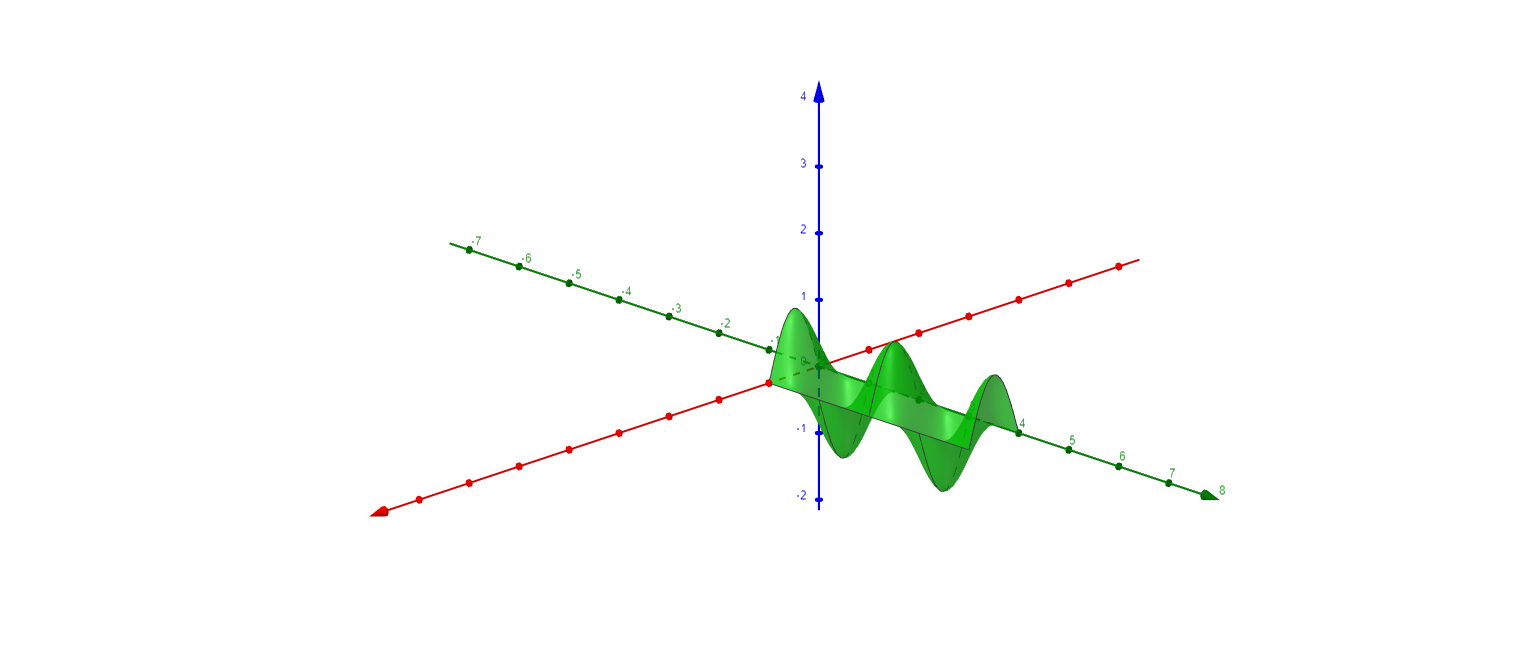
\includegraphics[width=.5\textwidth]{Figures/wave_solution_2.png}
        \end{figure}
        % \begin{figure}[H]
        %     \centering
        %     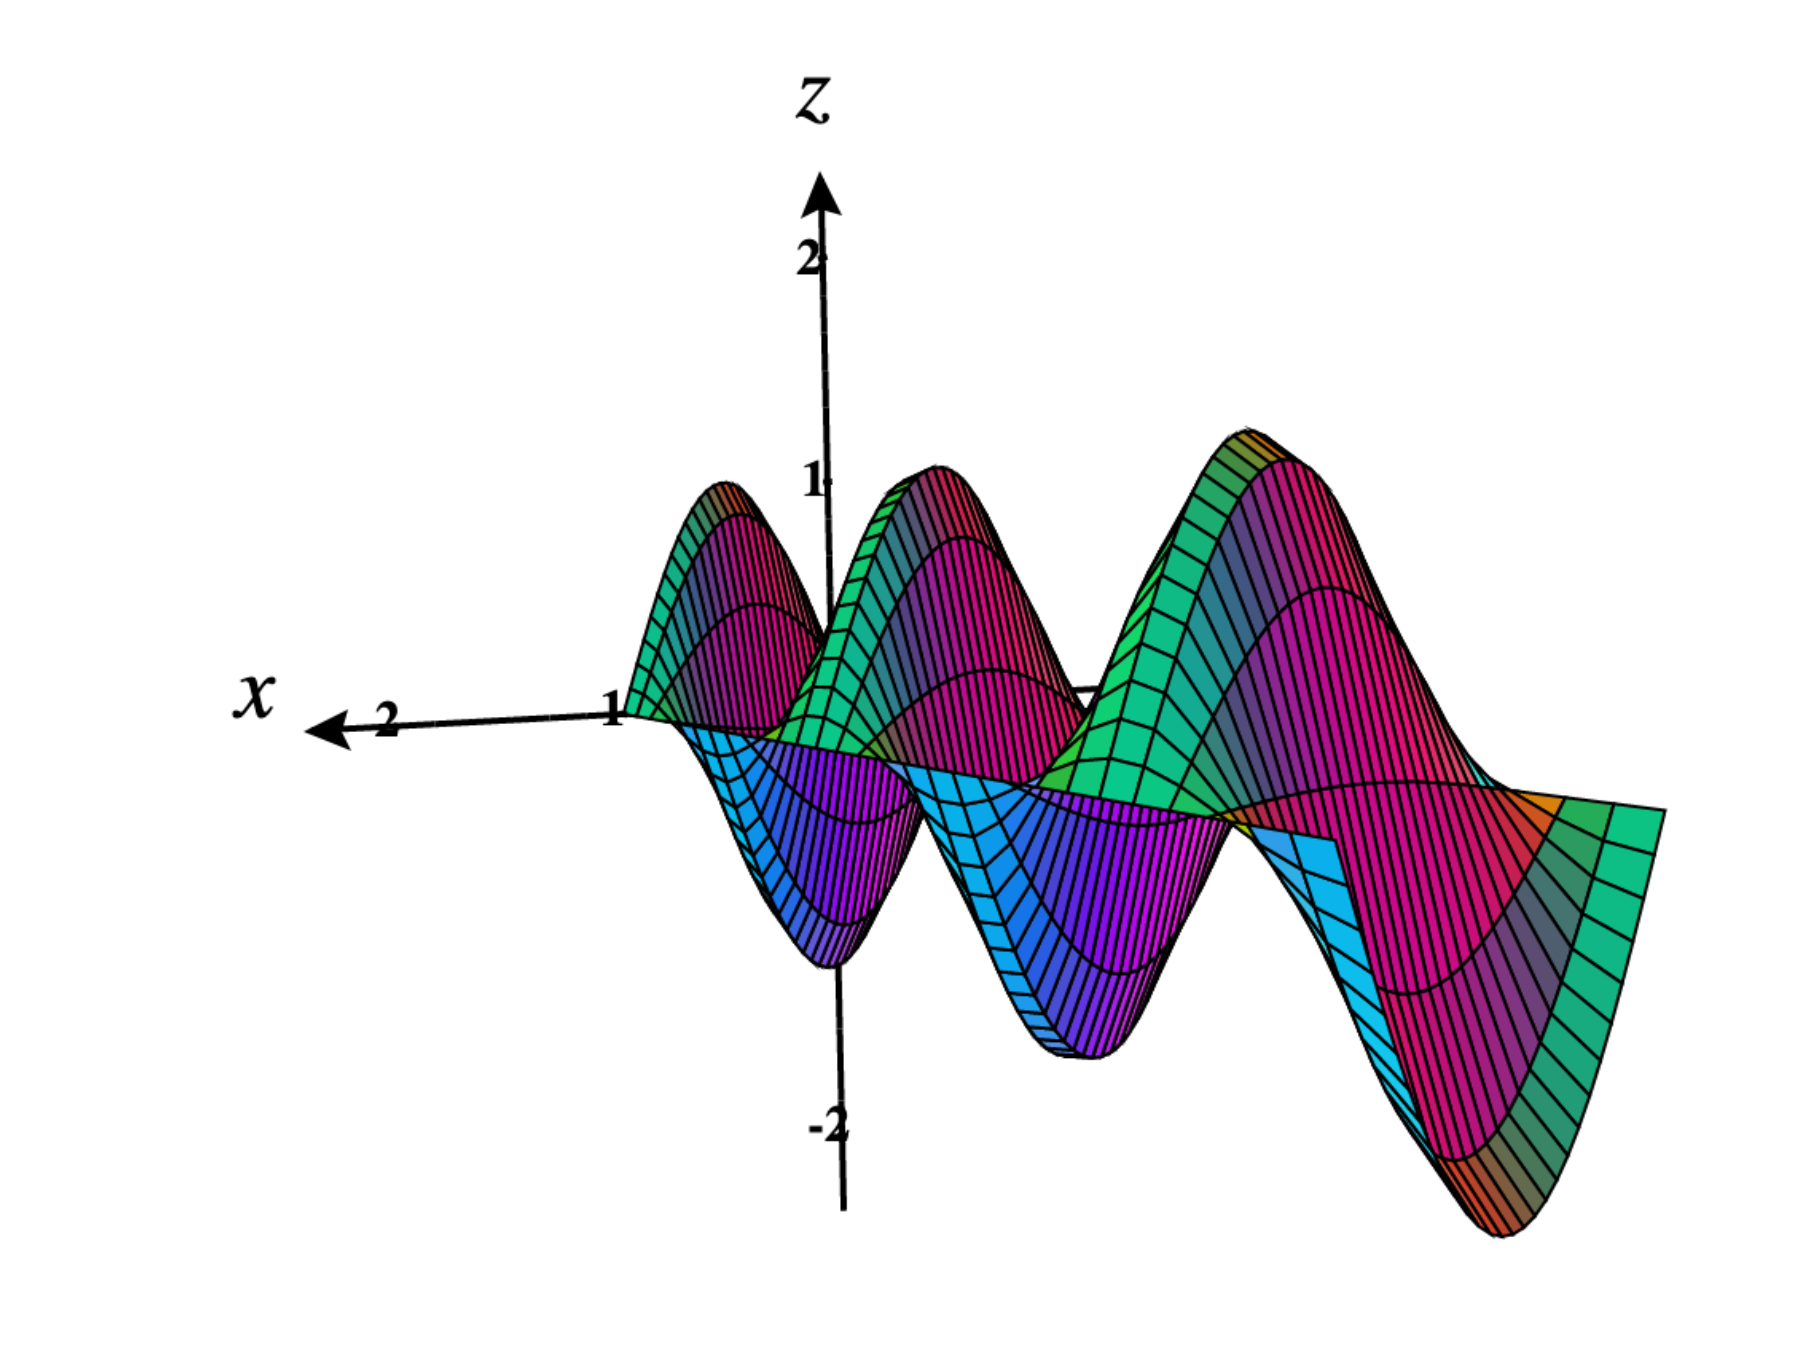
\includegraphics[width=.5\textwidth]{Figures/wave_solution.png}
        % \end{figure}
        \end{ex}

% \end{document}
